\documentclass{amsart}
\usepackage[utf8]{inputenc}

%\documentclass[a4paper,11pt]{amsart}

\input{000_setup}

\title[Area-Invariant Pedal-Like Curves]{Area-Invariant Pedal-Like Curves\\Derived from the Ellipse}
\author[D. Reznik]{Dan Reznik} 
\author[R. Garcia]{Ronaldo Garcia}
\author[H. Stachel]{Hellmuth Stachel}
%\date{June, 2020}
\date{May, 2021}

\begin{document}

\maketitle

\begin{abstract}
We study six pedal-like curves associated with the ellipse  which are area-invariant for pedal points lying on one of two shapes: (i) a circle concentric with the ellipse, or (ii) the ellipse boundary itself. Case (i) is a corollary of properties of Steiner's Curvature Centroid (Krümmungs-Schwerpunkt), proved in 1825. For case (ii) we prove area invariance algebraically. Explicit expressions for all invariant areas are also provided. Finally, we generalize the results for a class of smooth curves.

\vskip .3cm
\noindent\textbf{Keywords} ellipse, pedal, contrapedal, evolute, curvature centroid, invariance.
\vskip .3cm
\noindent \textbf{MSC} {53A04 \and 51M04 \and 51N20}
\end{abstract}


\section{Introduction}
\label{sec:intro}
Consider an ellipse $\mathcal{E}$ and a fixed point $M$. Let $\mathcal{E}_n$ denote the {\em negative-pedal curve} with respect to $M$ \cite{stachel2019-conics}, i.e., the envelope of lines $\mathcal{L}(t)$ through a point $P(t)$ on $\mathcal{E}$ and perpendicular to $P(t)-M$; see Figure~\ref{fig:npc-3}. This article was motivated by a recent result  \cite{garcia2020-deltoid}: $\mathcal{E}_n$ is a three-cusp area-invariant deltoid for all $M$ on $\mathcal{E}$; see Figure~\ref{fig:npc-3} (top right).

\begin{figure}
    \centering
    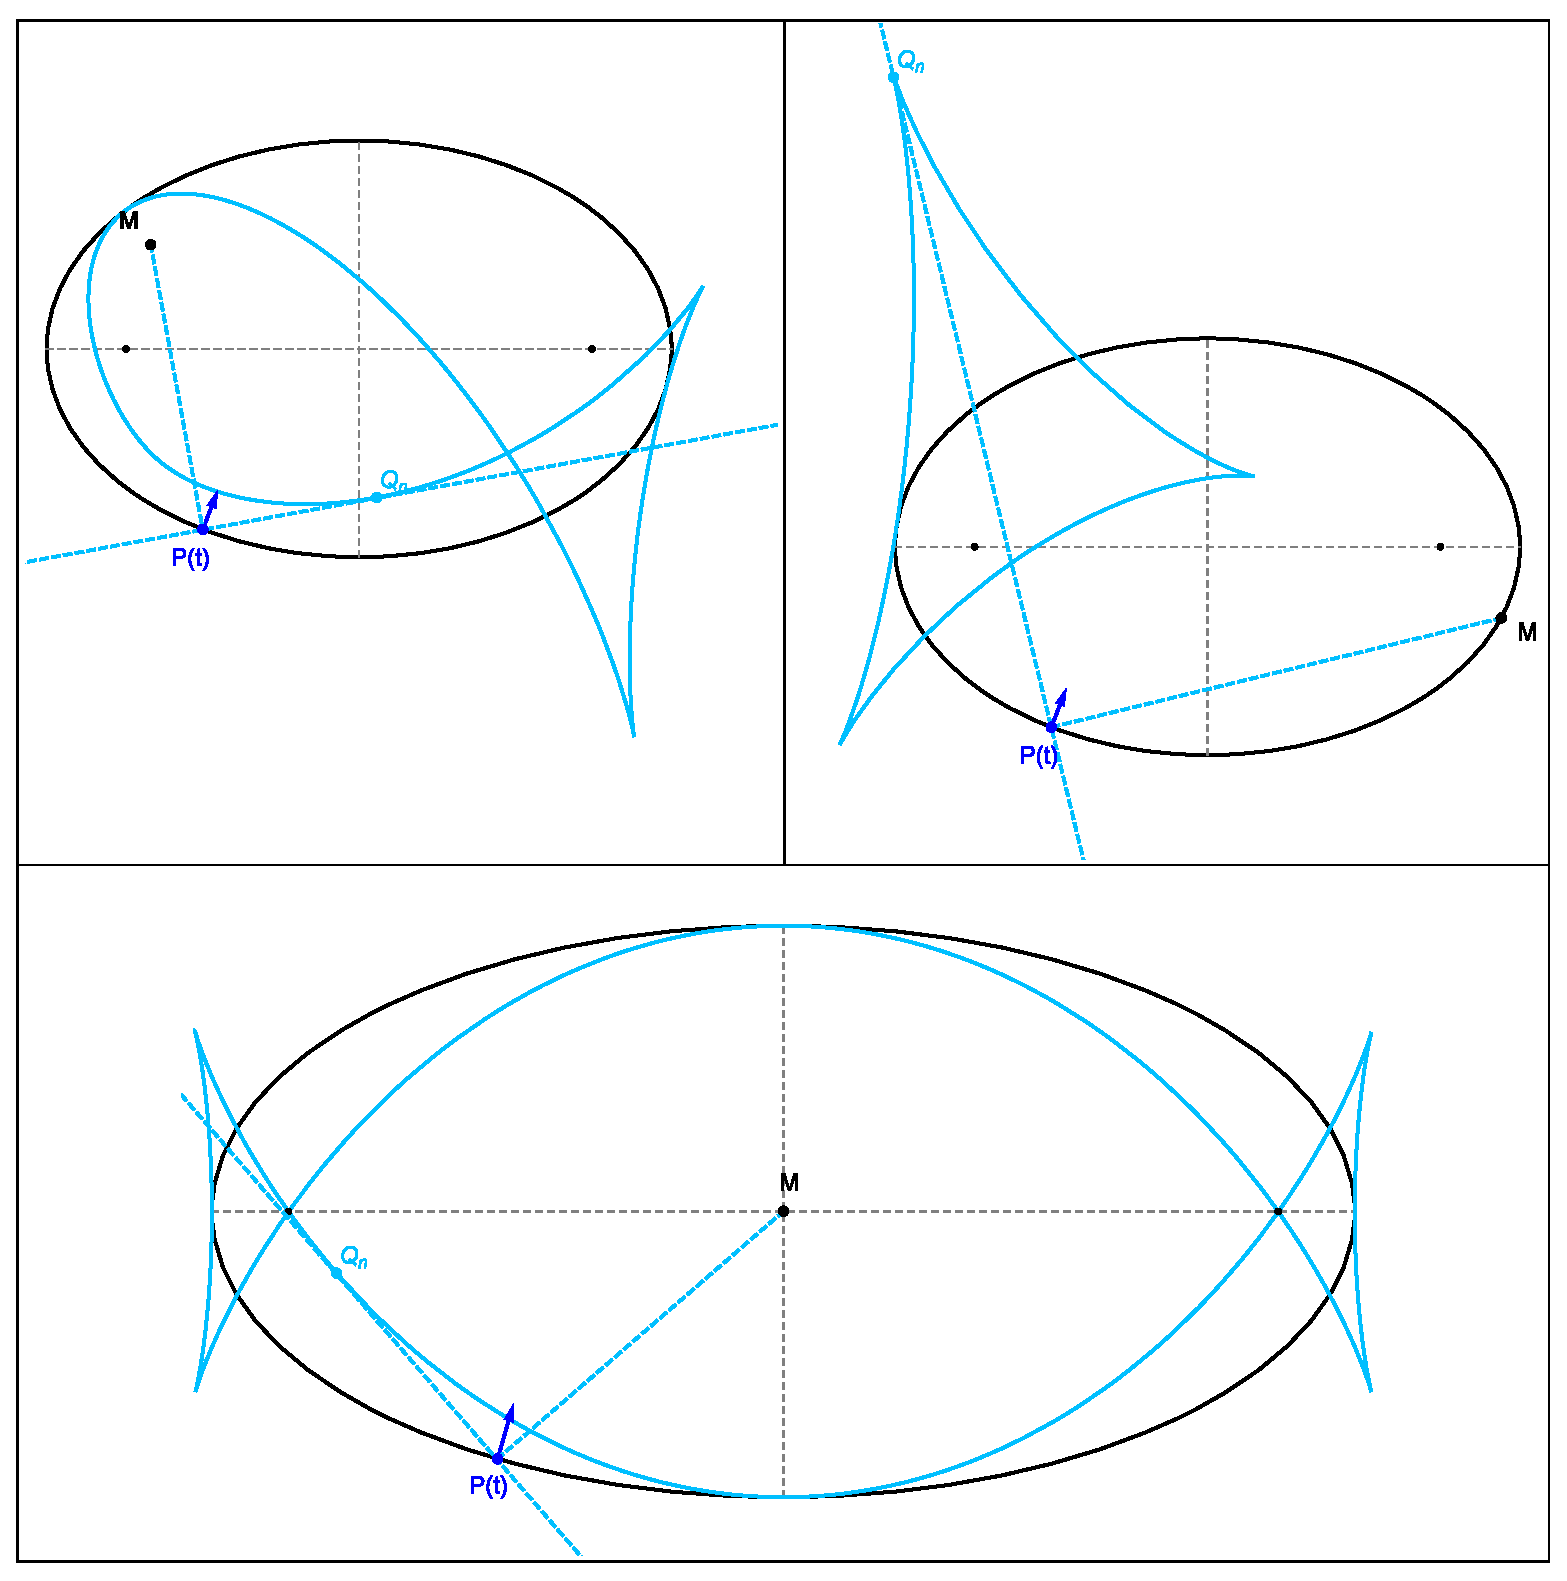
\includegraphics[width=\textwidth]{pics/0005_npc_3.eps}
    \caption{Examples of the Negative-Pedal Curve (light blue) of an ellipse (black) with respect to a point $M$. These are the envelope of lines through $P(t)$ on the ellipse, perpendicular to $P(t)-M$ ($Q_n$ is the tangent point). Three cases are shown, for $M$ (i) interior (top left), (ii) on the boundary (top right), and (iii) at the center (bottom) of the ellipse. For case (ii) the area of the curve is invariant for all $M$ \cite{garcia2020-deltoid}. Case (iii) yields Talbot's Curve \cite{mw} (in general it does not pass through the foci, but for the case shown, $a/b=2$, it does).} 
    \label{fig:npc-3}
\end{figure}

Let $\mathcal{E}_p$, $\mathcal{E}_c$ denote the {\em pedal}, and {\em contrapedal}, curves of $\mathcal{E}$ with respect to a point $M$ \cite{stachel2019-conics}; see Figures~\ref{fig:pedal-cp}. Recall the contrapedal of a plane curve is the pedal of the evolute \cite[Contrapedal]{mw}. For the ellipse, the evolute is a 4-cusp astroid \cite[Ellipse Evolute]{mw}; see Figure~\ref{fig:contrapedal}.  Additionally, define:

\begin{itemize}
    \item The {\em Rotated Pedal Curve} $\mathcal{E}_{\theta}$, the locus of foot $Q_{\theta}$ of a perpendicular dropped from $M$ onto the line through $P(t)$ oriented along a $\theta$-rotated tangent to the ellipse, Figure~\ref{fig:theta-mu}(left).
    \item The {\em Interpolated Pedal Curve} $\mathcal{E}_{\mu}$, the locus a point $Q_{\mu}=(1-\mu)Q_p+{\mu}Q_c$ ($\mu$ is a constant), i.e., an affine combination of pedal and contrapedal feet, Figure~\ref{fig:theta-mu}(right).
    \item The {\em Hybrid Pedal Curve} $\mathcal{E}^*$, the locus of the intersection $Q^*$ of $\mathcal{L}(t)$ with the line from $M$ to $Q_p$, Figure~\ref{fig:hybrid}.
    \item The {\em Pseudo Talbot Curve}\footnote{After the actual Talbot's Curve, shown in Figure~\ref{fig:npc-3} (bottom): the negative pedal curve of an ellipse with respect to its center $O$.} $\mathcal{E}^\dagger$, i.e., the Negative Pedal Curve of $\mathcal{E}^*$, Figure~\ref{fig:hybrid-npc}.
\end{itemize}

\begin{figure}
    \centering
    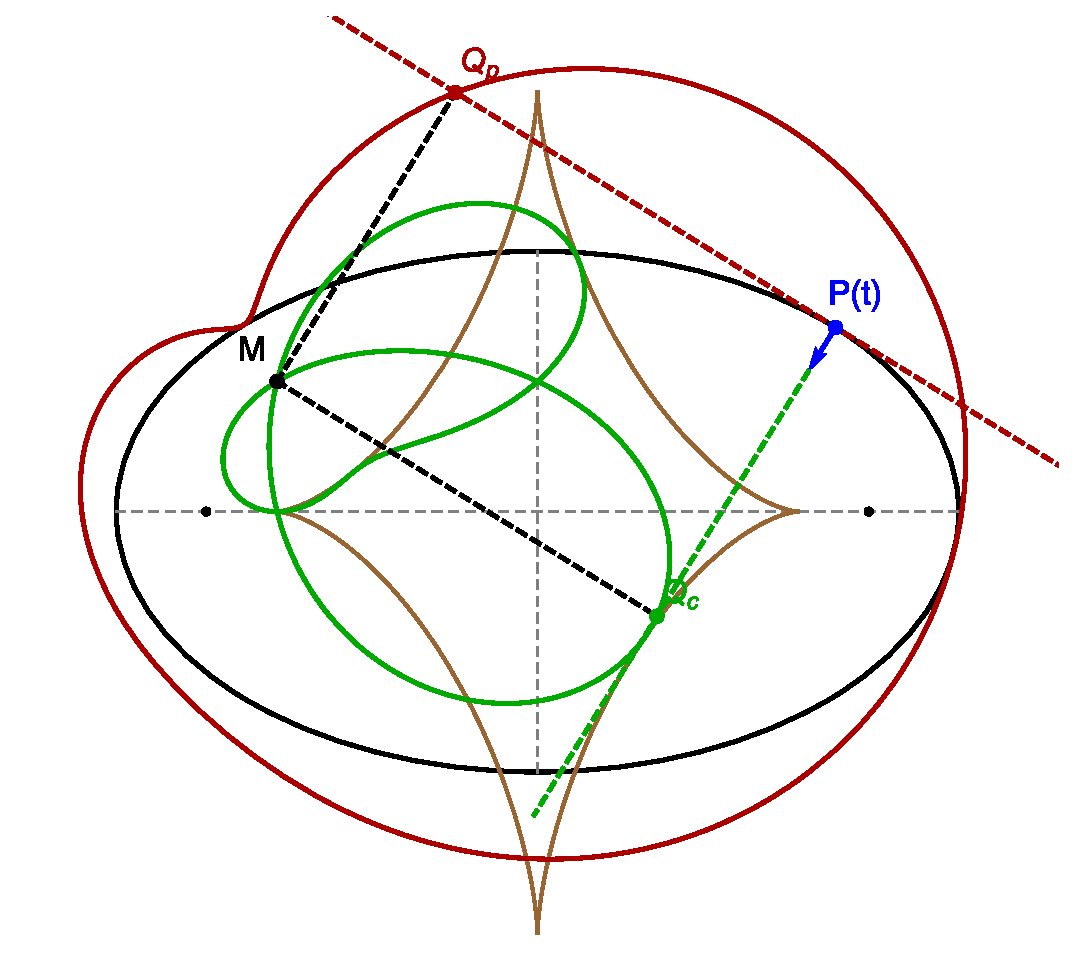
\includegraphics[width=.7\textwidth]{pics/0010_ped_cp.eps}
    \caption{The Ellipse Pedal Curve $\mathcal{E}_p$ (red) is the locus of the foot $Q_p$ of the perpendicular dropped from $M$ onto the line through $P(t)$ tangent to the ellipse. The Contrapedal Curve $\mathcal{E}_c$ (green) is the locus of foot $Q_c$ of the perpendicular dropped from $M$ onto the line through $P(t)$ normal to the ellipse. It can also be regarded as the pedal curve to the ellipse evolute (brown astroid).}
    \label{fig:pedal-cp}
\end{figure}

\begin{figure}
    \centering
    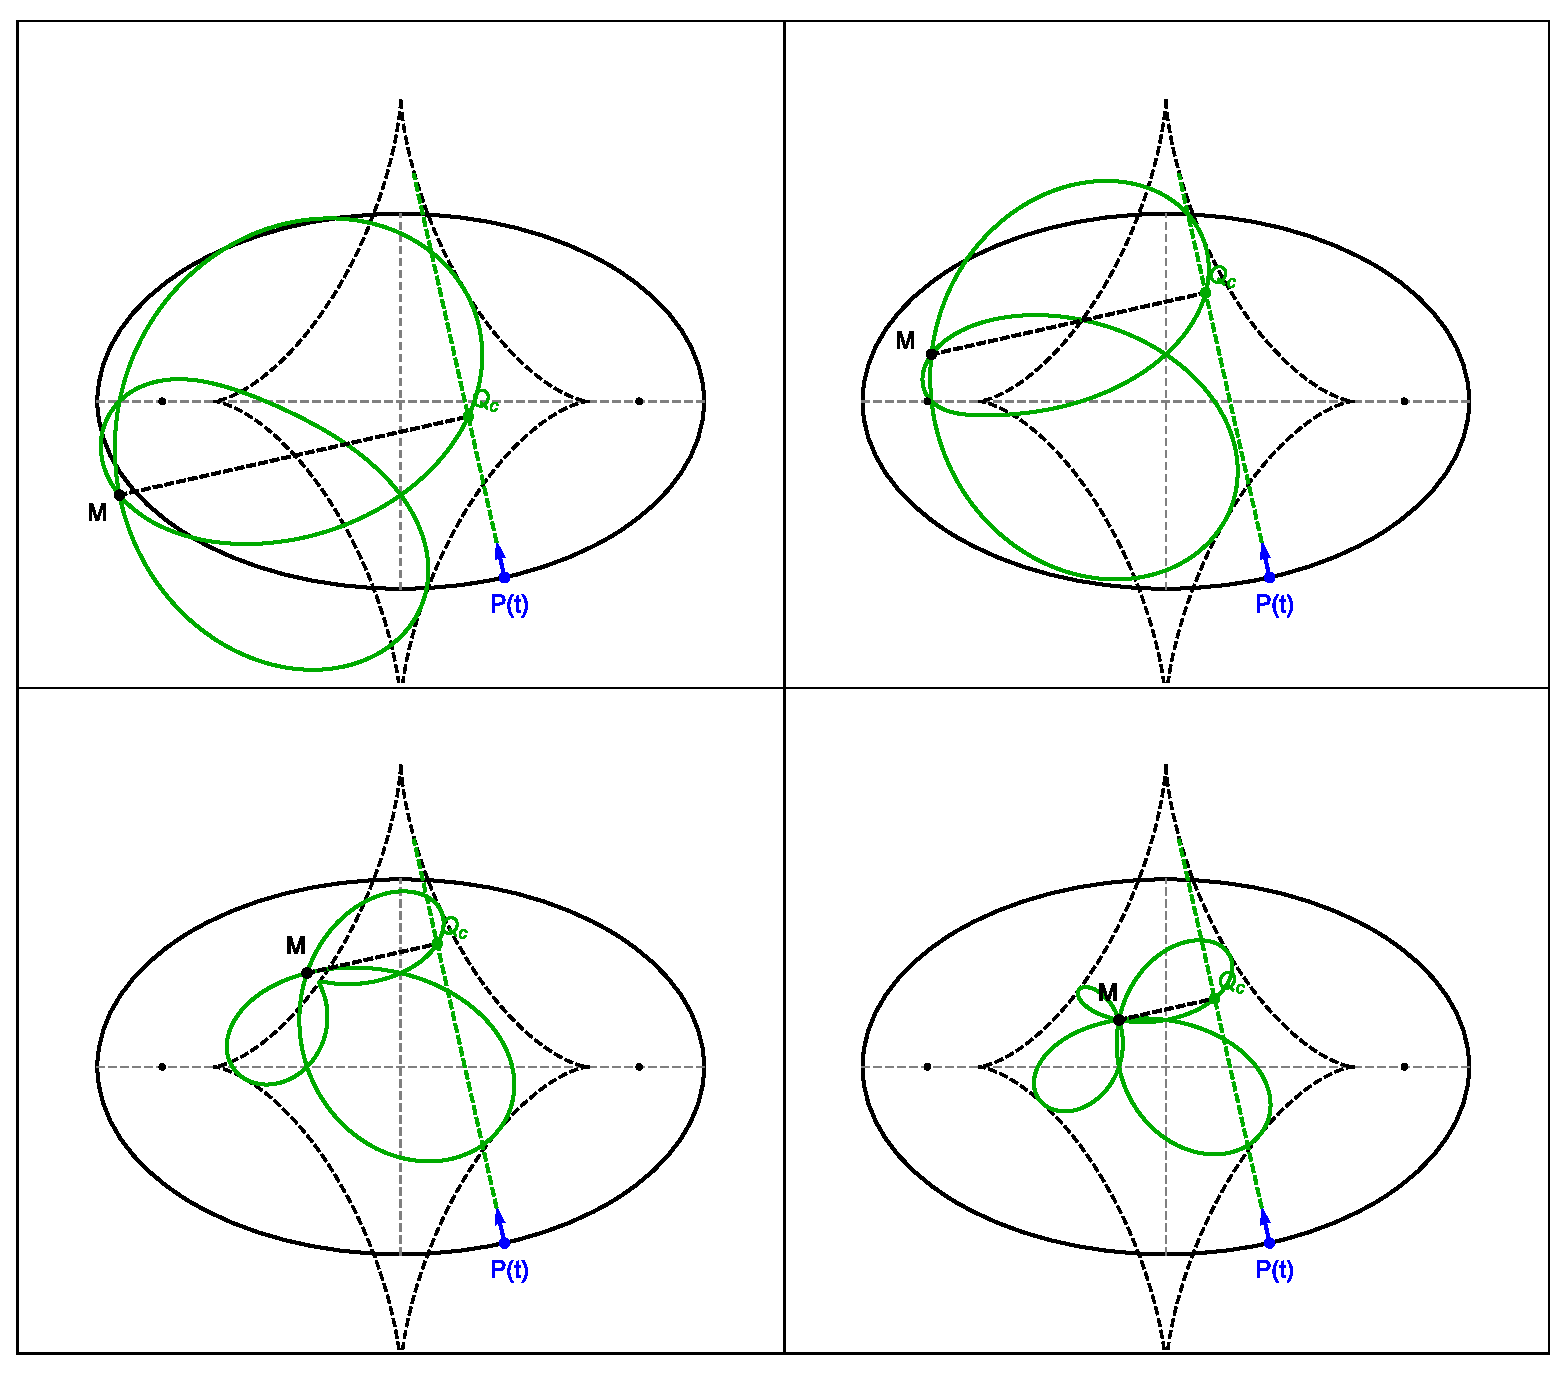
\includegraphics[width=\textwidth]{pics/0050_contrapedal_touchpts.eps}
    \caption{The ellipse Contrapedal Curve $\mathcal{E}_c$ (green) for four distinct positions of $M=[x_m,y_m]$. Notice the contrapedal is the pedal of the evolute (dashed black). We invite the reader to prove that (i) the curve's two self intersections (ignoring the one at $M$) always occur at $[x_m,0]$ and $[0,y_m]$ and (ii) that it touches the evolute at either 2 (top row) or 4 (bottom row) locations.}
    \label{fig:contrapedal}
\end{figure}

\begin{figure}
    \centering
    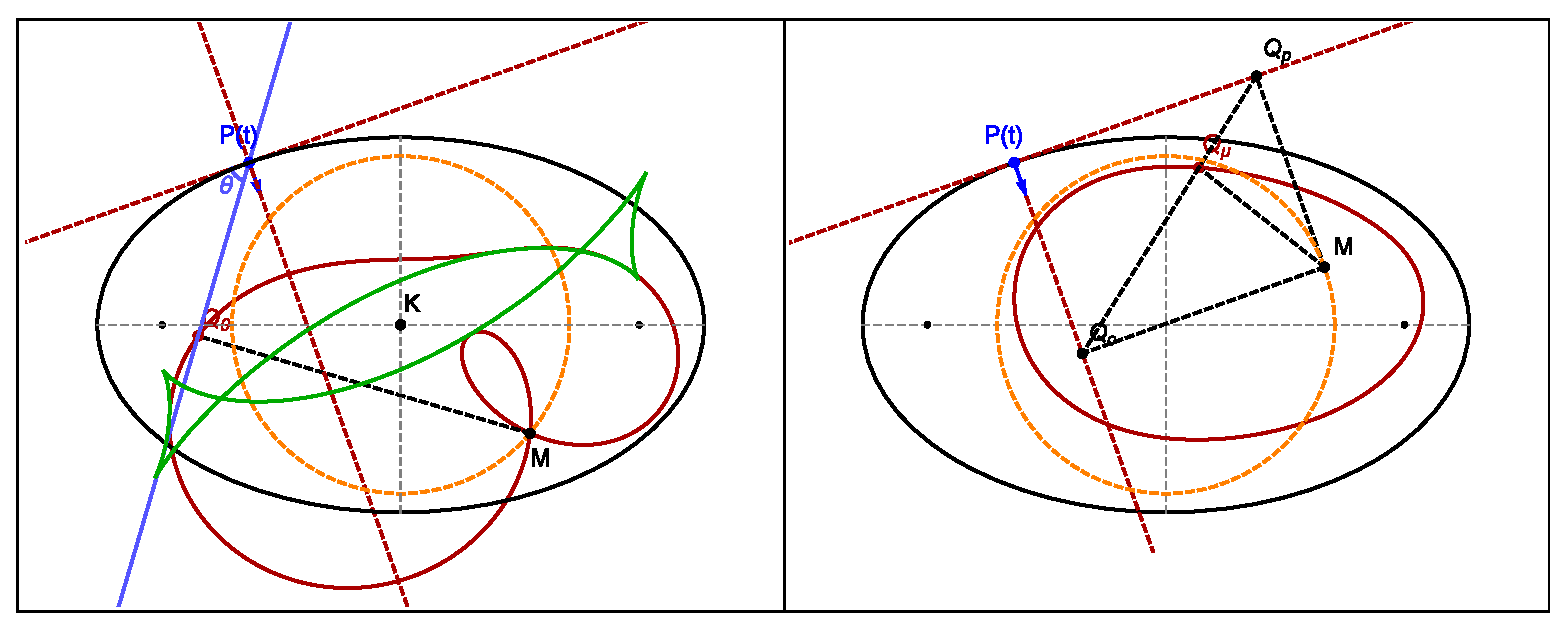
\includegraphics[width=\textwidth]{pics/0030_rot_mid.eps}
    \caption{\textbf{Left:} The rotated pedal curve $\mathcal{E}_{\theta}$ (red) is the locus of $Q_{\theta}$, the foot of a perpendicular dropped from $M$ onto a line through $P(t)$, along the $\theta$-rotated tangent (light blue), in this case $\theta=54^\circ$. $A_{\theta}$ is invariant for $M$ on a concentric circle (orange). Note $\mathcal{E}_0=\mathcal{E}_p$ and  $\mathcal{E}_{\pi/2}=\mathcal{E}_c$, and in general, $\mathcal{E}_\theta$ is the pedal curve with respect to the $\theta$-evolutoid (green), whose curvature centroid $K$ is stationary at $O$. \textbf{Right:} The interpolated pedal curve $\mathcal{E}_{\mu}$ (red) is the locus of $Q_{\mu}$, the affine combination of pedal $Q_p$ and contrapedal $Q_c$ feet, here $\mu=1/3$. $A_{\mu}$ is invariant provided $M$ lies on a concentric circle (orange).}
    \label{fig:theta-mu}
\end{figure}

Let $A$, $A_p$, $A_c$, $A_\theta$, $A_\mu$, $A^*$, and $A^\dagger$ denote the areas of $\mathcal{E}$, $\mathcal{E}_p$,
$\mathcal{E}_c$,
$\mathcal{E}_\theta$,
$\mathcal{E}_\mu$,  $\mathcal{E}^*$, and $\mathcal{E}^\dagger$, respectively. 

\subsection*{Main Results}

In Section~\ref{sec:review-steiner} we review a theorem by Jakob Steiner \cite{pamfilos2019-krummungs,steiner1838} concerning the Curvature Centroid (Krümmungs-Schwerpunkt) of polygons; a corollary is that $A_p$, $A_c$, and $A_{\theta}$ are invariant for $M$ along any circle concentric with $\mathcal{E}$. Furthermore, we prove $A_{\mu}$ also shares this property.

In Section~\ref{sec:explicit}, we derive explicit expressions for $A$, $A_p$, $A_c$, $A_\theta$, $A_\mu$ in terms of $\mathcal{E}$'s semi-axes $(a,b)$, $M$, $\mu$ and $\theta$. We also show that (i) $A_p-A_c=A$, and (ii) $A_p-A_\theta=A\sin^2\theta$.

In Section~\ref{sec:main-results} we prove that both $A^*$ and $A^\dagger$ are invariant for $M$ on $\mathcal{E}$. Finally, in Section~\ref{sec:epilogue}, we generalize area-invariance results to a large class of smooth curves. 

Appendix~\ref{app:general-evolutoids} contains  propositions supporting results related to ellipse evolutes and evolutoids (see \cite{jesus2015,jesus2014} for more details).
A table of all symbols used herein appears in Appendix~\ref{app:symbols}.

%\item Wherever $\mathcal{E}_p$ is tangent to $\mathcal{E}$, so is $\mathcal{E}^*$.
%\item $\mathcal{E}_c$ touches the ellipse evolute on either 2 or 4 points. \textcolor{red}{explicit conditions on $M$?}
% \item \textcolor{red}{ronaldo} $\mathcal{E}_c$ has two self-intersections at $(M_x,0)$, and  $(0,M_y)$.
    %\item \textcolor{red}{ronaldo} Let $C_{2,p}$ and $C_{2,c}$ denote the area centroids of $\mathcal{E}_p$ and $\mathcal{E}_c$, respectively. If $M$ moves along a circle, these move along ellipses.
    %\item The locus of $M$ for which $\mathcal{E}_p$ has a cusp is \textcolor{red}{...}





\section{Sturm and Steiner: Circular Area Isocurves}
\label{sec:review-steiner}
A 1823 Theorem by Sturm states that given a triangle, the area of the {\em pedal triangle} with respect to a point $M$ is constant for all $M$ on a circle centered on the circumcenter $X_3$ \cite[Thm. 7.28, page 221]{ostermann2012}, Figure~\ref{fig:sturm}.

\begin{figure}
    \centering
    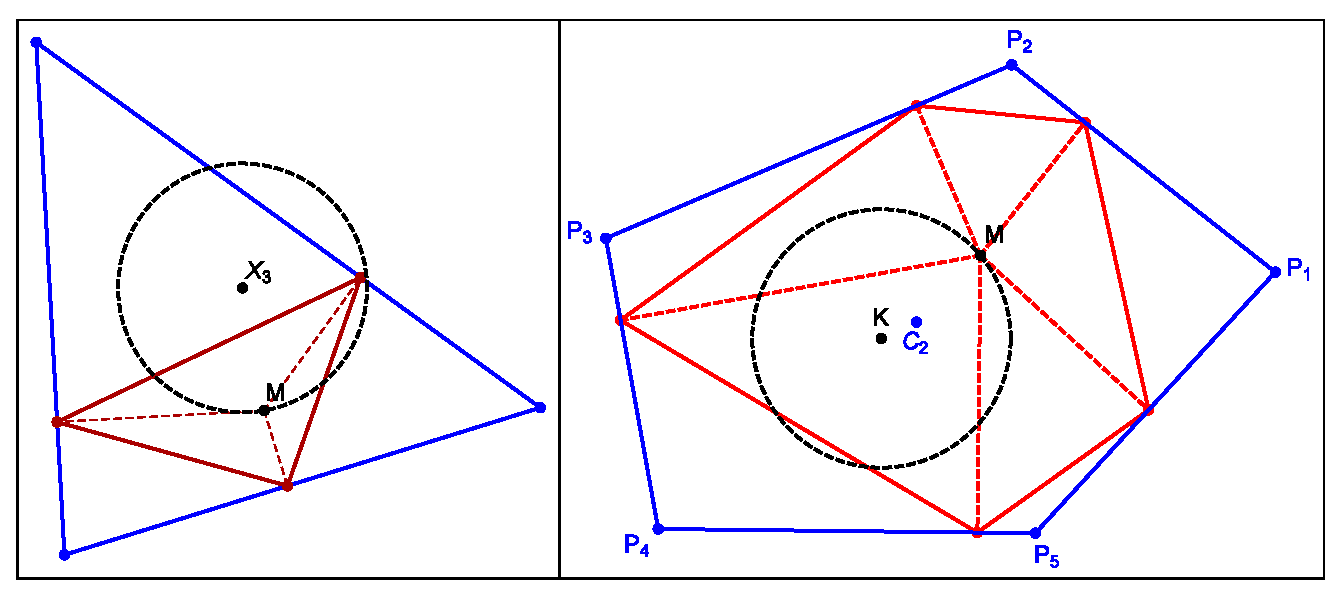
\includegraphics[width=\textwidth]{pics/0006_sturm_and_steiner.eps}
    \caption{\textbf{Left}: Sturm's Theorem (1823) states that the area of the pedal triangle (red) of a reference triangle (blue) is invariant for all points $M$ lying a circles (dashed black) centered on the circumcenter $X_3$. \textbf{Right}: in 1825, Steiner generalizes this to polygons: the area of the pedal polygon (red) to an N-gon (blue) is constant for all $M$ over a circle centered on $K$, the curvature centroid. $C_2$ denotes the polygon's center of area.}
    \label{fig:sturm}
\end{figure}

In 1825 Steiner generalized it as follows: given a polygon with vertices $P_i,i=1,{\ldots}N$, the area of its pedal polygon with respect to $M$ is invariant for $M$ on a circle centered on Steiner's {\em curvature centroid} $K$, given by \cite{steiner1838}:

\begin{equation*}
    K = \frac{\sum_i{\sin(2\theta_i) P_i}}{\sum_i{\sin(2\theta_i)}}
%    \label{eq:centroid-steiner}
\end{equation*}

\noindent where $\theta_i$ are the internal angles, $i=1,\cdots,N$. In the same publication Steiner also proves that the pedal polygon with respect to $K$ has extremal area. Note for $N=3$, $K=X_3$ as the latter has barycentrics of $\sin(2\theta_i)$ \cite{etc}. This is consistent with the fact that pedal polygons with respect to points on the circumcircle have constant area (in fact they have zero area, their vertices lie on the Simson line \cite[Simson Line]{mw}).

Steiner further generalized the above to the case of a closed plane curve $\mathcal{C}$, by approximating it with a polygon where $N{\rightarrow}\infty$. Let the {\em pedal curve} $\mathcal{C}_p$ of $\mathcal{C}$ with respect to a point $M$ be the locus of the foot of the perpendicular dropped from $M$ onto 
  the tangent at a point $P(t)$ to $\mathcal{C}$
  for all $t$; see Figure~\ref{fig:steiner-general}. With $N{\rightarrow}\infty$,
provided that the total curvature of $\mathcal{C}$ is non-zero (i.e., non-zero winding number), $K$ becomes \cite{steiner1838}:

\begin{equation}
    K = \frac{\int{\kappa(s) P(s).ds}}{\int{\kappa(s).ds}}
    \label{eqn:steiner-k}
\end{equation}

\noindent where $\kappa(s)$ is the curvature and $s$ is arc length. Referring to Figure~\ref{fig:steiner-general}, we recall a result by Jakob Steiner \cite{steiner1838}:  

\begin{theorem*}[Steiner, 1825]
The area of the pedal curve is constant for  points $M$ lying on circles centered on $K$.
%\label{thm:pedal}
\end{theorem*}

\begin{figure}
    \centering
    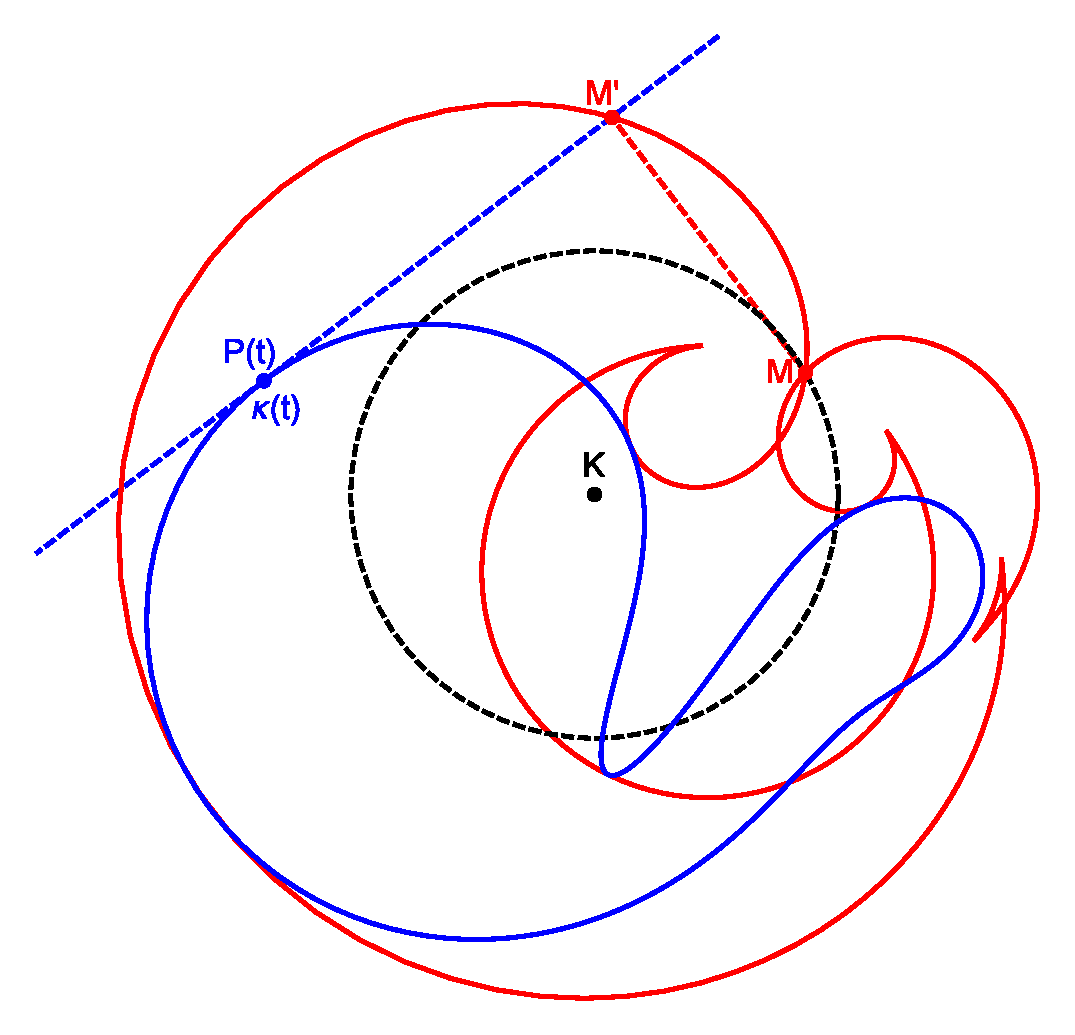
\includegraphics[width=.5\textwidth]{pics/0007_general_poly_steiner.eps}
    \caption{A generic closed curve $\mathcal{C}$ (blue) and its pedal curve (red), defined as the locus of the foot $M'$ of perpendiculars dropped from $M$
    onto the tangent to $\mathcal C$ at $P(t)$.
     The Steiner curvature centroid $K$ is obtained by averaging the curvature $\kappa(t)$ over all $P(t)$; see equation~\eqref{eqn:steiner-k}. The signed area of the pedal polygon is constant for $M$ lying in a circle centered on $K$.}
    \label{fig:steiner-general}
\end{figure}

From symmetry:

\begin{lemma}
For the ellipse and its evolute (an astroid), $K=O$.
%\label{lem:ellipse-k}
\end{lemma}

%Note: when expressed in line %coordinates, the cusps of the evolute %are regular. Specifically, cusps of the %evolute are inflection points of its %dual \cite{fischer2001,akopyan2007-conic%s}. 

Referring to Figure~\ref{fig:pedal-contrapedal}:

\begin{figure}
    \centering
    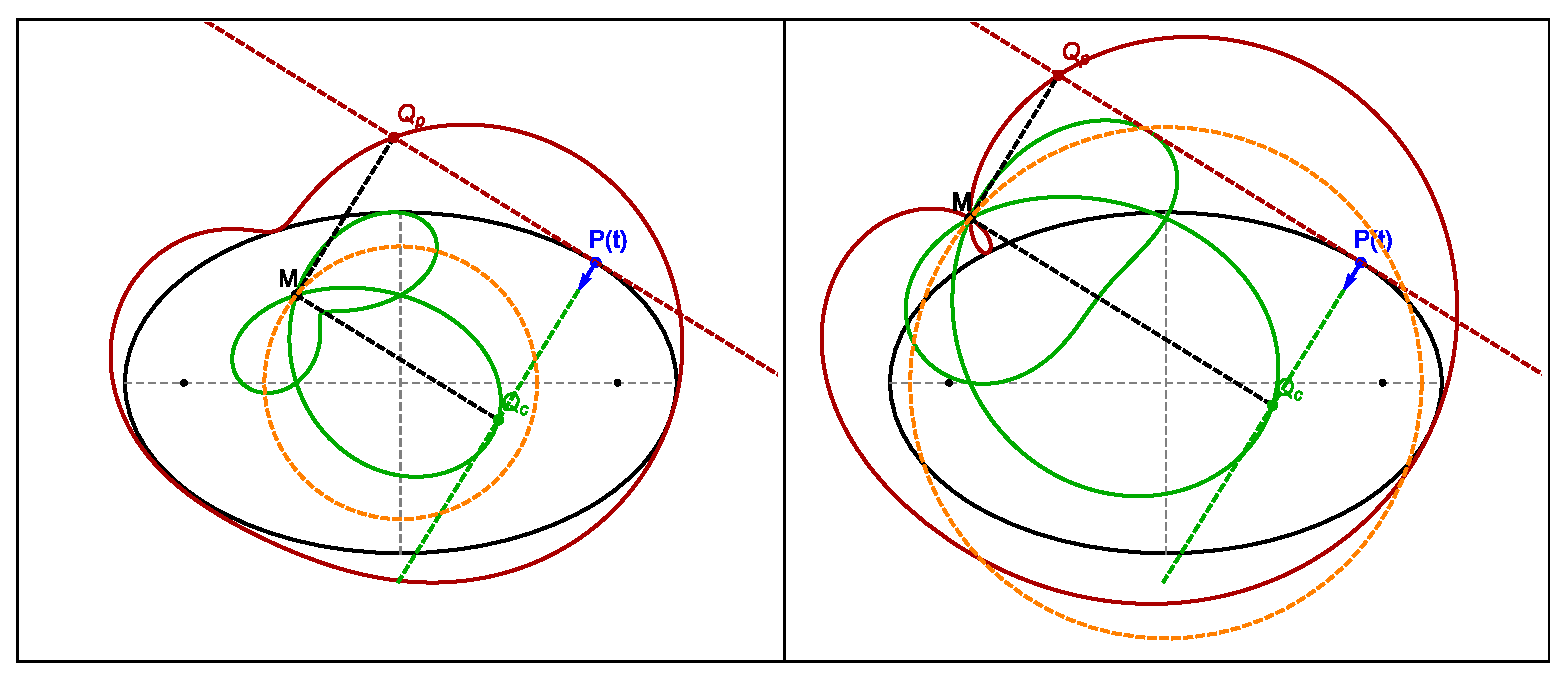
\includegraphics[width=\textwidth]{pics/0020_iso_areas.eps}
    \caption{\textbf{Left:} The areas $A_p$ (resp. $A_c$) of the Pedal Curve $\mathcal{E}_{p}$ (red) (resp. Contrapedal Curve $\mathcal{E}_{c}$, green) are invariant for all $M$ on a circle (orange) concentric with the ellipse. \textbf{Right:} An iso-area concentric circle (orange) of radius larger than the minor axis of the ellipse.}
    \label{fig:pedal-contrapedal}
\end{figure}

\begin{corollary}
The area $A_p$ of the pedal curve is invariant for $M$ on a circle concentric with $\mathcal{E}$.
\end{corollary}

As illustrated for an ellipse in Figure~\ref{fig:contrapedal}, in general, the contrapedal curve is the pedal curve with respect to the evolute \cite[Contrapedal Curve]{mw} and:

\begin{corollary}
The area $A_c$ of the contrapedal curve is invariant for $M$ on a circle concentric with $\mathcal{E}$.
\end{corollary}

Let the term $\theta$-evolutoid denote the envelope of $\theta$-rotated tangents to a curve; see Figure~\ref{fig:evolutoid}.

\begin{figure}
    \centering
    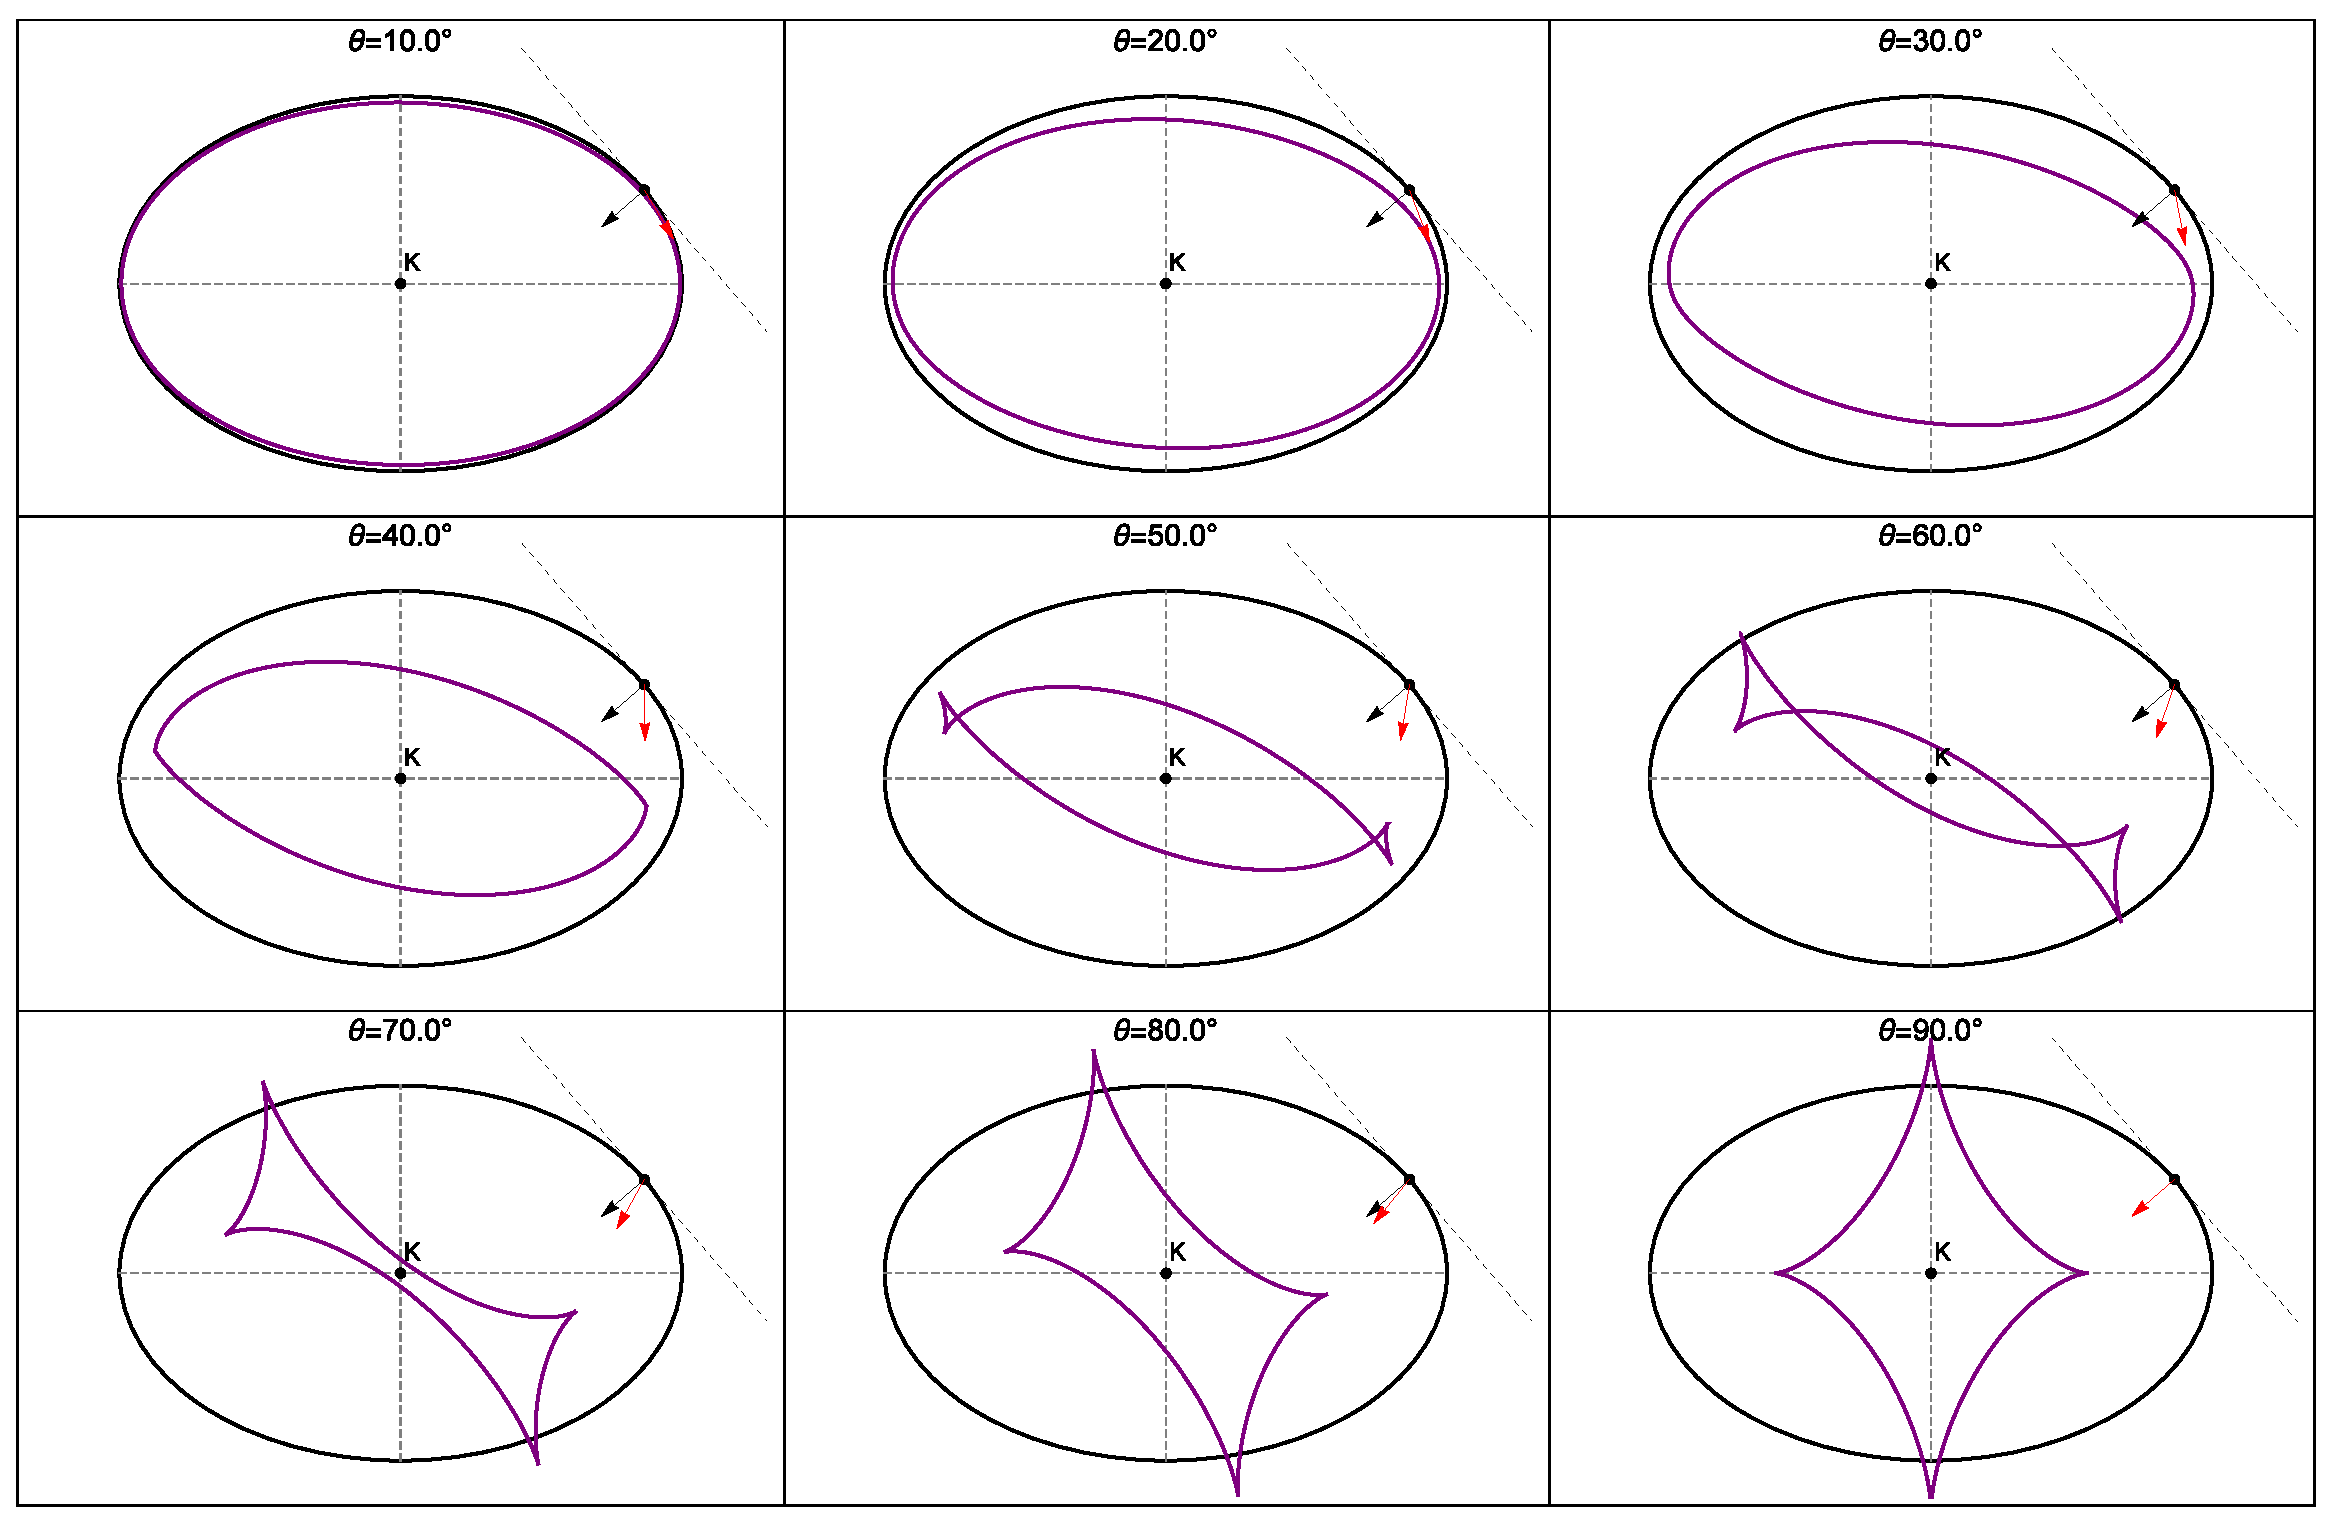
\includegraphics[width=\textwidth]{pics/0015_evolutoids.eps}
    \caption{The $\theta$-evolutoid \cite{jesus2015,jesus2014} (purple, envelope of tangents rotated by $\theta$) for an $a/b=1.5$ ellipse, $\theta=10,\ldots,90$ degrees. The bottom-right figure ($\theta=90^\circ$) is the ellipse evolute. Also shown are the normal (black arrow) and rotated tangent (red arrow) for a point in the 1st quadrant. Since these curves are centrally symmetric, the Steiner curvature centroid $K$ lies at the ellipse center.}
    \label{fig:evolutoid}
\end{figure}

\begin{lemma}
The $\theta$-evolutoid to an ellipse has $K=O$, for any $\theta$.  
\label{lem:evolutoid-k}
\end{lemma}

This stems from the fact that for all $\theta$, the $\theta$-evolutoid remains symmetric with respect to the origin $O$.

\begin{corollary}
The area $A_{\theta}$ of the rotated contrapedal curve is invariant for $M$ on a circle concentric with $\mathcal{E}$.
\end{corollary}

This stems from the fact that the rotated pedal curve $\mathcal{E}_{\theta}$ is the pedal with respect to a $\theta$-evolutoid and Lemma~\ref{lem:evolutoid-k}.

\begin{theorem}
The area $A_\mu$ of the interpolated pedal curve is invariant for $M$ on a circle concentric with $\mathcal{E}$.
\end{theorem}

\begin{proof}
Proposition~\ref{prop:amu-concave} in Section~\ref{sec:epilogue} shows that for any closed curve with non-zero total curvature (the denominator of Equation~\eqref{eqn:steiner-k}),  $A_{\mu}$ is a fixed linear function of $A_p$ and $A_c$. Since both $A_p$ and $A_c$ are constant for $M$ on circles centered on $K=O$, the result follows.
\end{proof}


\section{Explicit Areas}
\label{sec:explicit}
As before, let a point $P(t)$ on $\mathcal{E}$ be parametrized as $P(t)=[a\cos t,b\sin t]$. Define the {\em signed area} of a curve $\gamma$ as:

\begin{equation}
\mathcal{A}_\gamma=\frac{1}{2}\int_{\gamma}(x{dy}-y{dx}).
\label{eqn:area}
\end{equation}

%The support function of the ellipse is $h(t)=\sqrt{a^2\cos^2t+b^2\sin^2 t}$.

Referring to Figure~\ref{fig:evolutoid}, the $\theta$-evolutoid is the envelope of lines passing through $P(t)$ rotated with respect to the tangent vector $P'(t)$ by $\theta$. Its coordinates can be derived explicitly as

\begin{align*}
x_{\theta}(t)=& a\cos^{2}{\theta}\cos{t}
  + \frac {c^2 \sin^2  \theta 
		\cos^3   t  
	 }{a} - \frac {\sin t \sin   \theta
	  \cos  \theta    (   b^2\cos^2 t
		 +{a}^{2}   \sin^2 t )}{b} 
 \\
y_{\theta}(t)=&a\sin   \theta
\cos  \theta  \cos   t - \frac {c^2\sin{\theta} \cos^{2}t \left( b\cos
		t \cos  \theta  -a\sin  \theta
	  \sin t \right) }{ab}  \\
  +& \frac {
		\sin t   \left( b^2\cos^2   \theta 
	  -c^2 \sin^2  \theta  
		 \right)}{b}
%
\end{align*}

\noindent with $c^2=a^2-b^2$.

Let $\theta_0=\tan^{-1}\left(\frac{2ab}{{3}c^2}\right)$.

\begin{remark}
 The parametrization $[x_\theta(t), y_\theta(t)]$ of the $\theta$-evolutoid will   have 4, 2, or 0 singularities if
$\theta\in(\theta_0,\pi-\theta_0)$, $\theta\in\{\theta_0,\pi-\theta_0\}$, or $\theta\notin[\theta_0,\pi-\theta_0]$, respectively. Moreover, the ${\theta_0}$-evolutoid is singular at $t_1=\frac{3\pi}{4}$ and
	$t_2=  \frac{7\pi}{4}$.
	Here, a  point $t=t_0$ is called singular when $x'_\theta(t_0)=y'_\theta(t_0)=0$.
	These points correspond to real cusps of the curve.  
	In the implicit form,   a  $\theta$-evolutoid is given by $f^{-1}(0)$, and $f$ being a polynomial   function of degree 12.
\end{remark}

\begin{proposition}
The signed area $S_\theta$ of the 
$\theta$-evolutoid  of the ellipse $\mathcal E$ is given by:
%
\[S_{\theta}=\pi a b \cos^2\theta -\frac{  3 c^4\pi}{8 ab} \sin^2\theta\]
% \label{prop:aelipse}
\end{proposition}
\begin{proof}
Direct integration of Equation~\ref{eqn:area}.
\end{proof}

\begin{proposition}\label{prop:areapc}
The areas $A_p$ and $A_c$ of $\mathcal{E}_p$ and  $\mathcal{E}_c$ are given by: 

\begin{align}
A_p=&\frac{\pi}{2}\, \left( {a}^{2}+{b}^{2}+   x_0 ^{2}+  y_0^{2} \right) \label{eqn:ap} \\
A_c=&\frac{\pi}{2}\, \left( (a-b)^2 +   x_0 ^{2}+  y_0^{2} \right) \nonumber
\end{align}
where $M = [x_0,y_0]$. 
\end{proposition}


\begin{proof} Consider the ellipse parametrized by $P(t)=[a\cos t,b\sin t]$. Then it follows that
{\small 
\[\aligned
	\mathcal{E}_p(t)&=  \left[\frac{   a^2 x_0\sin^2 t -ab y_0\cos t\sin t+ab^2\cos t }{   b^2\cos ^2t+a^2\sin ^2t },  \frac{ b^2y_0\cos^2t -abx_0\cos t \sin t +a^2b\sin  t}{   b^2 \cos ^2t +a^2 \sin^2 t}\right]\\
	\mathcal{E}_c(t)&=\left[ \frac{\cos t( b^2x_0\cos t  + a b y_0 \sin t + a c^2\sin^2{t})}{ b^2 \cos ^2t +a^2 \sin^2 t},
	\frac{ \sin t( a b x_0 \cos t  - a^2 y_0\sin t   + b c^2\cos^2{t})  }{ b^2 \cos ^2t +a^2 \sin^2 t}\right]
	%\mathcal{E}_c(t)=&\left[ \frac{b^2x_0\cos ^2t  + \cos t\sin t %(aby_0+ac^2\sin{t})}{ b^2 \cos ^2t +a^2 \sin^2 t},
%	\frac{  a^2 y_0\sin ^2t + \cos t\sin %t(abx_0-b c^2\cos{t})  }{ b^2 \cos ^2t +a^2 \sin^2 t}\right]
	\endaligned \]
	}
 
Compute the above areas with Equation~\eqref{eqn:area}. The integrand will be a ratio of trigonometric polynomials. Evaluate the integrals by using classical residue theory \cite{ahlfors1979-complex}. Algebraic manipulation yields the claim.
\end{proof}

\noindent Note: formulas in \eqref{eqn:ap} and later are consistent with Steiner's result that the area of the pedal curve of $M$ is the sum of the area for $M=K$ and a term proportional to the square of $|MK|$ \cite[p.~47]{steiner1838}.

\begin{corollary}
$A_p-A_c=A$.
\label{cor:area-diff}
\end{corollary}

\noindent As shown in Section~\ref{sec:epilogue}, the above holds holds for all smooth curves.

The rotated pedal curve $\mathcal{E}_{\theta}$ is given by
$[X_\theta/\Delta,Y_\theta/\Delta]$ where:
{\small 
\begin{align*}
 X_\theta &=  - 
  \left(     {a}^{2}  \sin^2  t   
\cos^2\theta +\frac{1}{2} a b\sin \left( 2\,\theta
 \right)  \sin \left( 2\,t \right) +  b^2  \cos^2 t 
  \sin^2\theta  
 \right) {x_0} \\
&+ \frac{1}{2} \left(  (b^2
  \cos^2 t   - {a}^{2} \sin^2t)\sin \left( 2\,\theta \right)
  +ab\sin
 \left( 2\,t \right) \cos \left( 2\,\theta \right)   \right)  y_0
 \\
 &+ \frac{b}{4}(c^2 \cos t \sin(2t) + 2 a^2 \sin{ t} )\sin(2\theta) - a \cos t (b^2\cos^2\theta + c^2\, \sin^2 t\sin^2\theta) 
 \\
 Y_\theta&= \frac{1}{2} \left( (  b^2  \cos^2t -   a^2\sin ^2{t} )  \sin(2\theta)+ a b  \sin (2t)  \cos(2  \theta)       \right)  x_0\\
 &+ \left(  (    a^2 \sin ^2{t}-b^2\cos^2t) \cos^2\theta   +\frac{1}{2} a b  \sin(2\theta)     \sin(2 t)  - a^2  \sin ^2{t}\right)  y_0\\
 &+  \frac{c^2}{4}  \left(2b \cos t\sin^2\theta+ a  \sin {t}   \sin(2\theta)    \right)  \sin(2 t) 
  -\frac{ab}{2}\left(2a \cos^2\theta  \sin {t}   +b \cos{t}  \sin(2\theta)  \right)
   \\
 \Delta&={b}^{2}   \cos^2 t +{a}^{2}\sin^2t
\end{align*}
}

\begin{proposition}
The area $A_\theta$ of the rotated pedal curve is given by

%\aligned A(P_M)=&\frac{\pi}{2}\, \left( {a}^{2}+{b}^{2}+   x_0 ^{2}+  y_0^{2} \right)\\
\[ A_\theta=\frac{\pi}{2}\, \left(     {a}^{2}+b^2-2\,ab\sin^2\theta + x_0^{2}+y_0^{2} \right) \]
\end{proposition}

\begin{proof}
Similar to Proposition \ref{prop:areapc}.
\end{proof}

\begin{corollary}
$A_p-A_\theta=A\sin^2\theta$.
\end{corollary}

\begin{proposition}
\label{prop:interpol}
The area $A_\mu$ of $\mathcal{E}_{\mu}=(1-\mu)\mathcal{E}_p+\mu \mathcal{E}_c$ is given by:

\begin{align*} A_{\mu}=& \left(2\,{a}^{2}-3\,ab+2\,b^{2}+2\,x_0^{2}+2\,y_0^{2} \right) \pi\,{\mu}^2 -2\,\left( (a-b)^2  +x_0^{2}
+y_0^{2} \right) \pi\,\mu \\
+&\frac{1}{2}\left( a^2+b^2 +x_0^{2}+y_0^{2} \right) \pi\\
  =&(1-2\mu)[(1-\mu) A_p-\mu A_c]+\mu(1-\mu)A. 
\end{align*}

 
\end{proposition}

\begin{proof}
Similar to Proposition \ref{prop:areapc}. 
\end{proof}

\section{Area Invariance of Hybrid and Pseudo Talbot Curves}
\label{sec:main-results}
As defined in Section~\ref{sec:intro}, let (i) the Hybrid Pedal Curve $\mathcal{E}^*$ be the locus of the intersection $Q^*$ of $\mathcal{L}(t)$ with the line from $M$ to $Q_p$, Figure~\ref{fig:hybrid}, and (ii) the Pseudo Talbot Curve $\mathcal{E}^\dagger$ be  the Negative Pedal Curve of $\mathcal{E}^*$, Figure~\ref{fig:hybrid-npc}. Here we prove their area invariance over all $M$ on $\mathcal{E}$.

\begin{theorem}
	The area $A^*$ of $\mathcal{E}^*$ is invariant for all $M$ on $\mathcal{E}$ and given by:
	\[ A^*= \frac{\pi  (3a^4+2a^2b^2+3b^4)}{2 a b}=\frac{\pi(3\delta^2+5a^2b^2)}{2 a b},\;\; \delta=\sqrt{a^4-a^2b^2+b^4}
	\]
%\label{thm:area-hybrid}
\end{theorem}

\begin{proof}

Let $P(t)=[a\cos{t},b\sin{t}]$ be a point on $\mathcal{E}$. By definition (Section~\ref{sec:intro} and  Figure~\ref{fig:hybrid}), $\mathcal{E}^*$ is defined as the intersection of lines
\[ M+ uP'(t)^{\perp}\;\;\; \text{and}\;\;\; P(t)+v (M-P(t))^{\perp}.\]

\noindent Let $M=[x_0,y_0]$ and $\mathcal{E}(t)=[x^*(t),y^*(t)]$. Straightforward calculation leads to:

{\small
\begin{align*}
x^*(t)=&\frac{
-b\left(3{a}^{2}+{b}^{2}+4{y_0}^{2}\right)\cos{t}
+4{a}{b}{x_0}\cos{2{t}}
-b c^2 \cos{3{t}}
+4{a}{x_0}{y_0}\sin{t}
+4{b}^{2}{y_0}\sin{2{t}}
}{
4\left(a{y_0}\sin{t}+b{x_0}\cos{t}-{a}{b}\right)
}\\
y^*(t)=&\frac{
-a\left({a}^{2}+3{b}^{2}+4{x_0^{2}}\right)\sin{t}
+4{a}^{2}{x_0}\sin{2{t}}
-a c^2\sin{3{t}}
+4{b}{x_0}{y_0}\cos{t}
-4{a}{b}{y_0}\cos{2{t}}
}{
4\left(a{y_0}\sin{t}+b{x_0}\cos{t}-{a}{b}\right)
}
\end{align*}
}

\noindent where $c^2=a^2-b^2$. Integrating Equation~\ref{eqn:area} over $\mathcal{E}^*(t)$ yields the claim.
\end{proof}

\begin{figure}
    \centering
    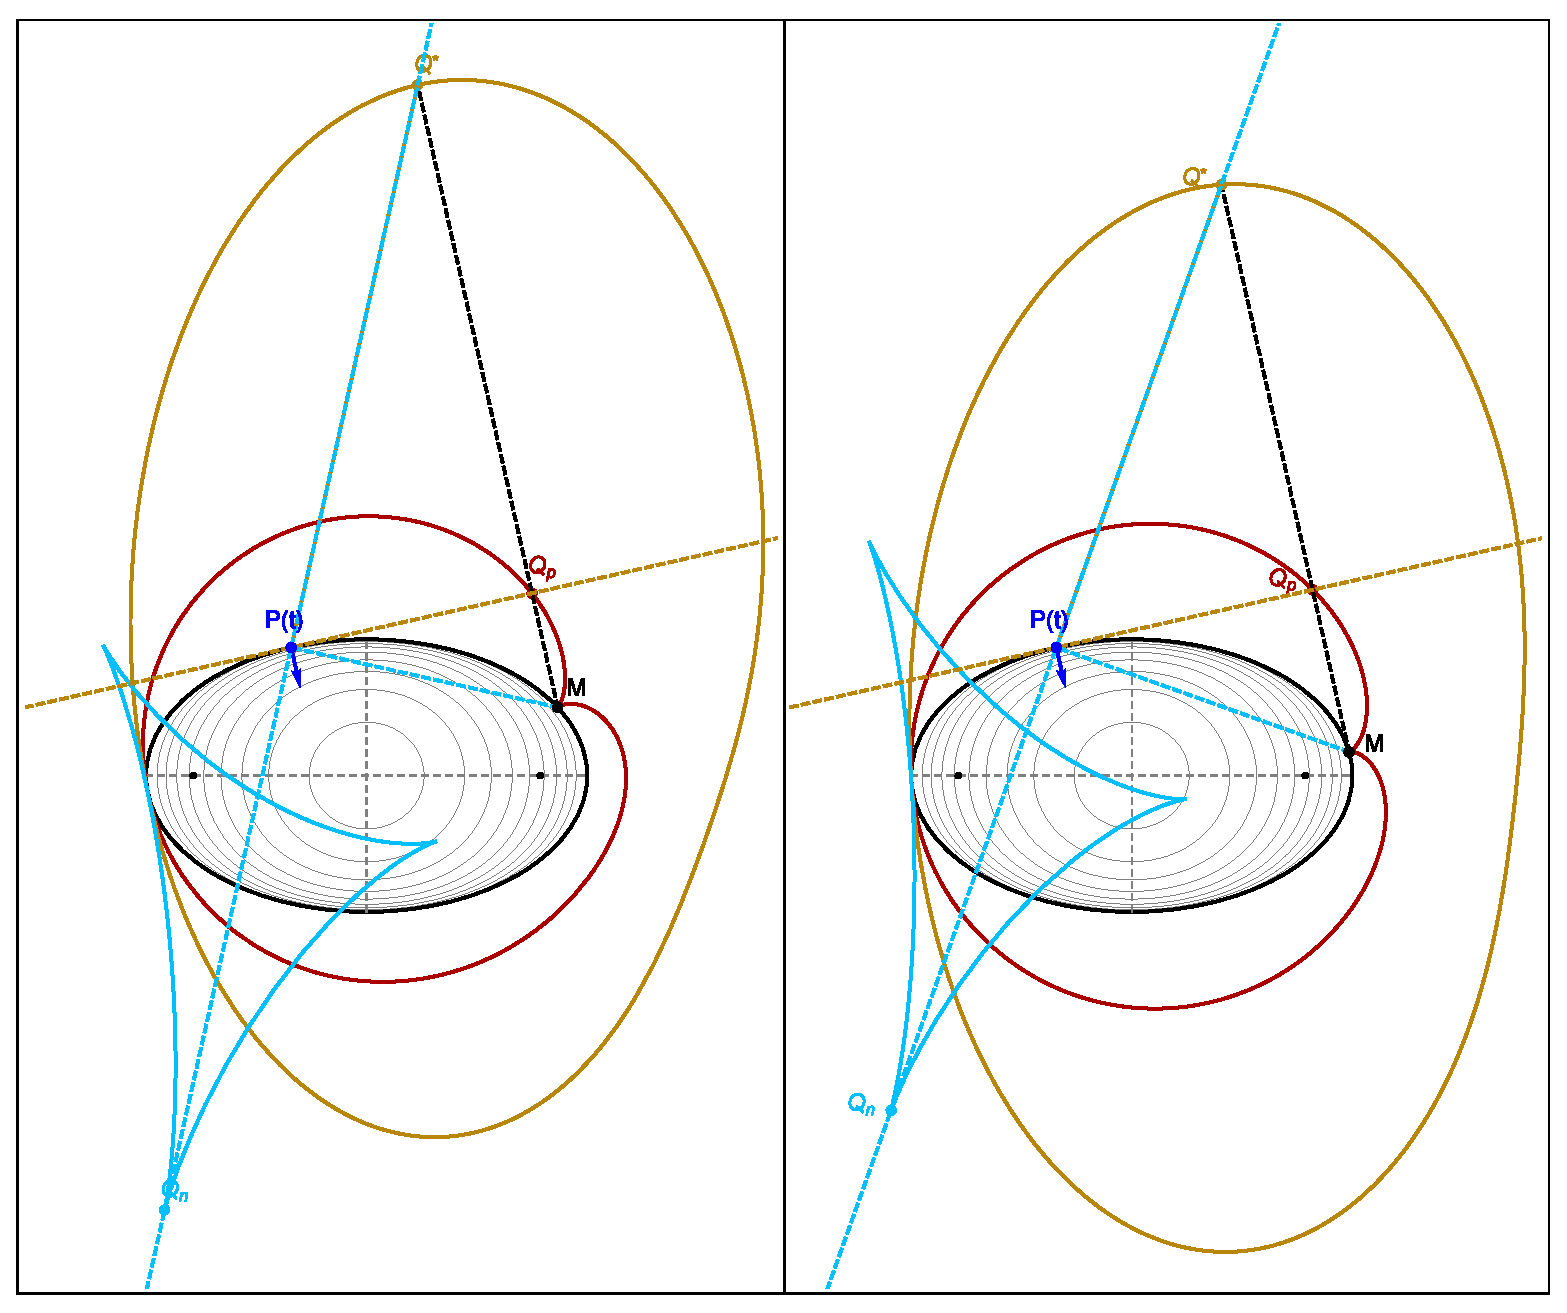
\includegraphics[width=\textwidth]{pics/0040_hybrid_curve.eps}
    \caption{The Pedal $\mathcal{E}_p$ (red) and Hybrid Pedal $\mathcal{E}^*$ (light brown), and Negative-Pedal $\mathcal{E}_n$ (light blue) Curves of the ellipse $\mathcal{E}$ (black) shown for two positions of $M$. $\mathcal{E}^*$ is the locus of the intersection $Q^*$ of (i) the line through $P(t)$ perpendicular to $P(t)-M$ and (ii) line $M{Q_p}$ (note $\mathcal{E}_p$ is the locus of $Q_p$). For both left and right pictures (indeed for all $M$ on the ellipse), areas $A_n,A^*$ are constant, although that of $\mathcal{E}_p$ varies. Also shown are iso-curves of constant $A^*$ inside the ellipse; these are high-order rational curves. $\mathcal{E}^*$ is unstable when $M$ is exterior to $\mathcal{E}$.}
    \label{fig:hybrid}
\end{figure}

\begin{theorem}
The area $A^\dagger$ of $\mathcal{E}^\dagger$ is invariant for all $M$ on $\mathcal{E}$ and given by:
	
	\[ A^\dagger=  -  \frac {\pi\, \left( 3\,{a}^{4}+2\,{a}^{2}{b}^{2}+3\,{b}^{4}
 \right)  \left( {a}^{2}-2\,ab-{b}^{2} \right)  \left( {a}^{2}+2\,ab-{
b}^{2} \right) }{8 a^{3} b^{3}}
	\]
%\label{thm:area-talbot}
\end{theorem}

\begin{proof}
Recall $\mathcal{E}^\dagger$ is the negative pedal curve of $\mathcal{E}^*$ (Section~\ref{sec:intro} and Figure~\ref{fig:hybrid-npc}). For $M=[a\cos u,b\sin u]$ on the ellipse, the coordinates $[x^\dagger,y^\dagger]$ of $\mathcal{E}^\dagger$ can be derived explicitly:

{\small  
\begin{align*}
x^{\dagger}(u)=&\frac{\left(c^4(2\cos(2t) - \cos(4t)) - (a^2 - 3b^2)(a^2 + b^2)\right)\cos{u} }{4 a b^2} - \frac{2c^4 \sin^3t \cos{t} \sin{u}}{a b^2}\\
&+ \frac{(a^2 + b^2)(b^2-c^2\sin^2{t}  )\cos{t}}{a b^2}\\
y^{\dagger}(u)=&-\frac{2c^4 \sin{t} \cos^3{t}\cos{u}}{a^2b} - \frac{(c^4(2\cos(2t) + \cos(4t)) - (3a^2 - b^2)(a^2 + b^2))\sin{u}}{ 4a^2b}\\
&+\frac{  (a^2 + b^2)(c^2 \cos^2{t}    + a^2)\sin{t}}{a^2 b}
\end{align*}
}

Integrating Equation~\eqref{eqn:area} for the above yields the claimed results.
\end{proof}

\begin{figure}
    \centering
    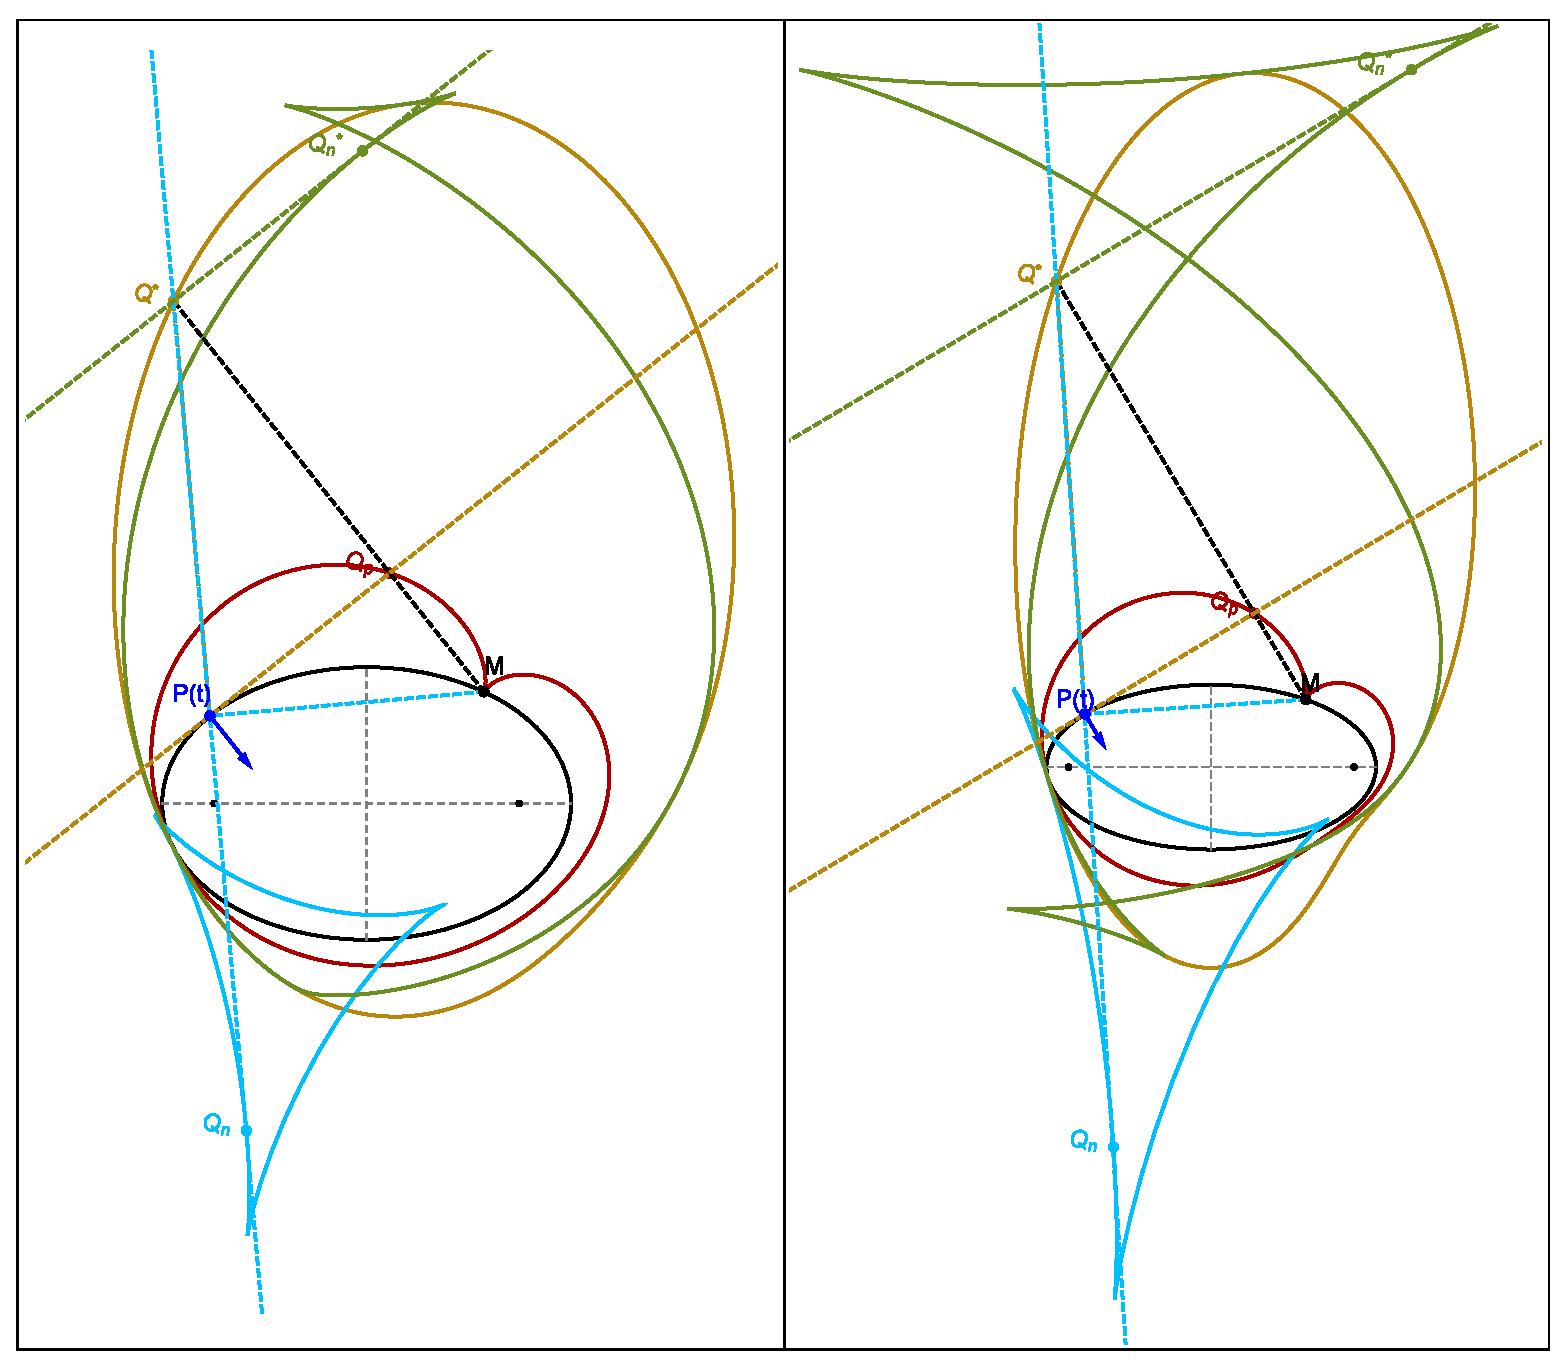
\includegraphics[width=\textwidth]{pics/0060_hybrid_npc.eps}
    \caption{The pedal, negative pedal, hybrid pedal $\mathcal{E}^*$, and pseudo-Talbot curve $\mathcal{E}^\dagger$ (negative pedal curve of $\mathcal{E}^*$) are shown red, light blue, brown, and olive green, respectively, for aspect ratios $a/b$ of $\mathcal{E}$ of 1.5 (left) and 2.0 (right), respectively. Notice that for the former case $\mathcal{E}^\dagger$ has two cusps, and in the latter 4. Excluding the pedal curve, all other 3 are area-invariant for $M$ on $\mathcal{E}$, and are all tangent to $\mathcal{E}$ at the point where the normal goes through $M$.}
    \label{fig:hybrid-npc}
\end{figure}




\section{Generalizing area-invariance to   smooth curves}

 Consider a plane  curve $\mathcal{C}(t)=[x(t),y(t)]$ defined by a support function $h$:

\begin{align}
x(t)=&h(t)\cos t-h'(t)\sin t \label{eqn:support}\\
y(t)=&h(t)\sin t+h'(t)\cos t \nonumber
\end{align}
%

\begin{remark*} In terms of a support function $h(t)=\sqrt{a^2\cos^2{t}  + b^2\sin^2{t}}$
the  ellipse is parametrized by:
\[  \left[ \frac{a^2\cos{t} }{ \sqrt{a^2\cos^2{t}  + b^2\sin^2{t}}}, \frac{b^2\sin{t}}{\sqrt{a^2\cos^2{t}  + b^2\sin^2{t}}} \right]\]
\end{remark*}

Let $M=(x_0,y_0)$ be a fixed point. Referring to Equation~\ref{eqn:support}, the pedal of $M$ is given by

\begin{equation}\label{eq:pedal-suporte}
 P_M(t)= [  x_0 \sin^2 t + \left( h(t) -y_0\sin
 t    \right) \cos t, \left( h(t) -{  x_0}\,\cos t  
   \right) \sin t +   y_0\cos^2 t ].
\end{equation}


The contrapedal of $M$ (intersection of the line $M+s \mathcal{C}'(t)$ and the normal line $\mathcal{C}(s)+u\mathcal{C}'(t)^{\perp}$) is given by

\begin{equation}\label{eq:contrapedal-suporte}
C_M(t)=  [ x_0  \cos^2t   +y_0\cos t
 \sin t -h'(t) \sin t , y_0 \sin^2t
 +x_0\cos t \sin t 
	 + h'(t) \cos t]
.
\end{equation}

Below is a generalization of Corollary~\ref{cor:area-diff}.


\begin{proposition}
For all smooth curves, the following holds:
	\[A(P_M)-A(C_M)=A(\mathcal{C})\]
	\label{prop:darea}

\end{proposition}

\begin{proof}
Obtain the signed areas for the above curves above via integration by parts of  Equation~\ref{eqn:area}. Algebraic manipulation yields the claim.
In fact, 
{\small  
\begin{align}
A(P_M)=& \frac{\pi}{2}(x_0^2+y_0^2)- \left(\int_0^{2\pi}\!\!\!\!\!\!h(t)\cos t dt\right) x_0- \left(\int_0^{2\pi}\!\!\!\!\!\!h(t)\sin t dt \right) y_0+\frac{1}{2}  \int_0^{2\pi}\!\!\!\!\!\!h(t)^2 dt\nonumber \\
A(C_M)=& \frac{\pi}{2}(x_0^2+y_0^2)- \left(\int_0^{2\pi}\!\!\!\!\!\!{h(t)\cos{t}dt}\right) x_0- \left(\int_0^{2\pi}\!\!\!\!\!\!h(t)\sin t dt \right) y_0+\frac{1}{2}\int_0^{2\pi}\!\!\!\!\!\!h^\prime(t)^2 dt \label{eqn:apm-acm}\\
A(\mathcal{C})=& \frac{1}{2}\int_0^{2\pi}\!\!\!\!\!(h(t)^2-h^{\prime}(t)^2)dt\nonumber
%
\end{align}
}
\end{proof}

%\begin{corollary}
%For any plane curve with vanishing signed area, $A(P_M)=A(C_M)$
%\end{corollary}

\begin{corollary} The family of isocurves of $A(P_M)$ and $A(C_M)$ are circles centered at
	
\begin{align*}
K_0=\left[  	\frac{1}{\pi} \int_0^{2\pi}\!\!\!\!\! h(t)\cos t \,dt,	\frac{1}{\pi} \int_0^{2\pi}\!\!\!\!\! h(t)\sin t \, dt\right]
\end{align*}
	
	
\end{corollary}
 
\begin{proof}  Consider the mean $K_0=\frac{1}{2\pi}\int_0^{2\pi}\mathcal{C}(t)dt$ of the curve $\mathcal{C}$ given by Equation \eqref{eqn:support}. Integration by parts leads to the result stated. Expressions of the areas $A(P_M)$ and $A(C_M)$ given in Equation \eqref{eqn:apm-acm} shows that the isocurves are cirles centered at $K_0$.
\end{proof}

\begin{remark}
For convex curves,  $K_0$ coincides with the   centroid of Steiner $K$ given by Equation \eqref{eqn:steiner-k}. In fact, using the parametrization  of the curve $\mathcal{C}$ given by Equation \eqref{eqn:support} it follows that
$ds= |h(t)+h''(t)|dt$ and $k(t)=1/(h(t)+h''(t))$. Integration by parts leads to the result.
\end{remark}

\begin{proposition} Let $P_{ {\theta }M}$ be the pedal of $M$ with respect to the curve $\mathcal{C}_\theta$.  For any convex curve $\mathcal{C}$ we have that:
	\[A(P_M)-A(P_{ {\theta }M})=\sin^2\theta A(\mathcal{C})\]
	
	\end{proposition}

\begin{proof} Similar to   that of Proposition \ref{prop:darea}.
\end{proof}

Referring to Figure~\ref{fig:interp-concave} and generalizing Proposition~\ref{prop:interpol}:

%\begin{proposition}
%\label{prop:amu}
%Let $\mathcal{C}_\mu=\mu P_M+(1-\mu)C_M$
	
%	Then, for $\mu\ne \frac{1}{2}$  the area isocurves of $\mathcal{C}_\mu$ are circles centered on $K$.
	
%	For  $\mu=\frac{1}{2}$,  the area isocurves of $\mathcal{C}_{\frac{1}{2}}$ are independent of the point $M$.
%\end{proposition}

%\begin{proof} Similar to the that of Proposition \ref{prop:darea}.
%	In fact, 
%	\begin{align*}
%	\mathcal{C}_\mu=&(2\mu-1)^2\left[   \frac{\pi}{2}(x_0^2+y_0^2)- \left(\int_0^{2\pi}\!\!\!\!\!\!h(t)\cos t dt\right) x_0- \left(\int_0^{2\pi}\!\!\!\!\!\!h(t)\sin t dt \right) y_0\right]\\
%	+&\frac{\mu^2}{2}  \int_0^{2\pi}\!\!\!\!\!\!h(t)^2 dt +\frac{(3\mu-1)(\mu-1)}{2}  \int_0^{2\pi} \!\!\!\!\!\!h^\prime(t)^2 dt.
%	\end{align*}
	
%	For $\mu=\frac{1}{2}$, it follows that $\mathcal{C}_{\frac{1}{2}}=\frac{1}{2}(M+\mathcal{C})$.\end{proof}

%\begin{corollary}
	
%	\begin{align*}
%	A(\mathcal{C}_\mu)=&(2\mu-1)\left( \mu A(P_M)+(1-\mu)A(C_M)\right)\\
%	+&\frac{\mu}{2}  \int_0^{2\pi}\!\!\!\!\!\!h(t)^2 dt+\frac{(\mu-1)(2\mu-1)}{2} \int_0^{2\pi}\!\!\!\!\!\! h^\prime(t)^2 dt  
%\end{align*}
%\end{corollary}

\begin{proposition}
\label{prop:amu-concave}
For any smooth regular closed curve $\mathcal{C}$ with non-zero rotating index, the isocurves of $A(\mathcal{C}_\mu)$ are circles centered on $K$.
In fact, \[A(\mathcal{C}_\mu) =(1-2\mu)[(1-\mu) A(P_M)-\mu A(C_M)]+\mu(1-\mu)A(\mathcal{C}).\]
\end{proposition}

\begin{proof}
Consider a smooth regular closed curve $\mathcal{C}(t)=[x(t),y(t)]$ parametrized by Equation \eqref{eqn:support}. Let $P_M(t)$ be the pedal and $C_M(t)$ be the contrapedal   curves in relation to $M$ given by Equations \eqref{eq:pedal-suporte} and \eqref{eq:contrapedal-suporte}.
Let $\mathcal{C}_\mu=(1-\mu) P_M+{\mu}C_M$.
 	
 	Computing   the area of $\mathcal{C}_{\mu}$ integrating Equation \eqref{eqn:area} and  using that
 	\begin{align*}
 	 \int_0^{2\pi} h''(t)\cos t\; dt &=-\int_0^{2\pi} h(t)\cos{t} \;  dt,\;\;\;
 	     \int_0^{2\pi} h''(t)\sin t \;dt =-\int_0^{2\pi} h(t)\sin{t}\;dt  \\ 
 	   \int_0^{2\pi} h'(t)\cos t\; dt &=\int_0^{2\pi} h(t)\sin{t} \;  dt, \;\;\;
 	     \int_0^{2\pi} h'(t)\sin t \;dt =-\int_0^{2\pi} h(t)\cos{t}\;dt  \\
 	      \int_0^{2\pi} h''(t)h(t)dt &=-\int_0^{2\pi}(h'(t))^2dt,\; \;
 	\end{align*}
the result follows, after   algebraic manipulations.
\end{proof}

\begin{remark*} When $\int_0^L k(s)ds=0$, or equivalently the rotating index of the curve is zero, the Steiner curvature centroid $K$ is not defined. In this case the pedal and contrapedal area isocurves will be either parallel lines or independent of $M$.
\end{remark*}

\begin{example} Consider the non convex smooth curve 
\[ 
\mathcal{C}(t)= [  2 \cos t -\frac{1}{4}\sin( 2t) + \frac{3}{10}\cos(2t),
\sin{t} + \frac{3}{4}\cos(2t)] \] 
The curvature centroid of $\mathcal{C}$ is $K=[0.1823\ldots, 0.01943\ldots]$. The linear centroid
$[\int xds/\int ds, \int yds/\int ds]$ is the point $[0.1387\ldots, -0.2504\ldots ] $ and the center of mass $[\int xdxdy/\int dxdy, \int ydxdy/\int dxdy]$ is $[12/95, 7/19]=[0.1263\ldots, -0.3684\ldots]$.
 
\end{example}


\begin{figure}
    \centering
    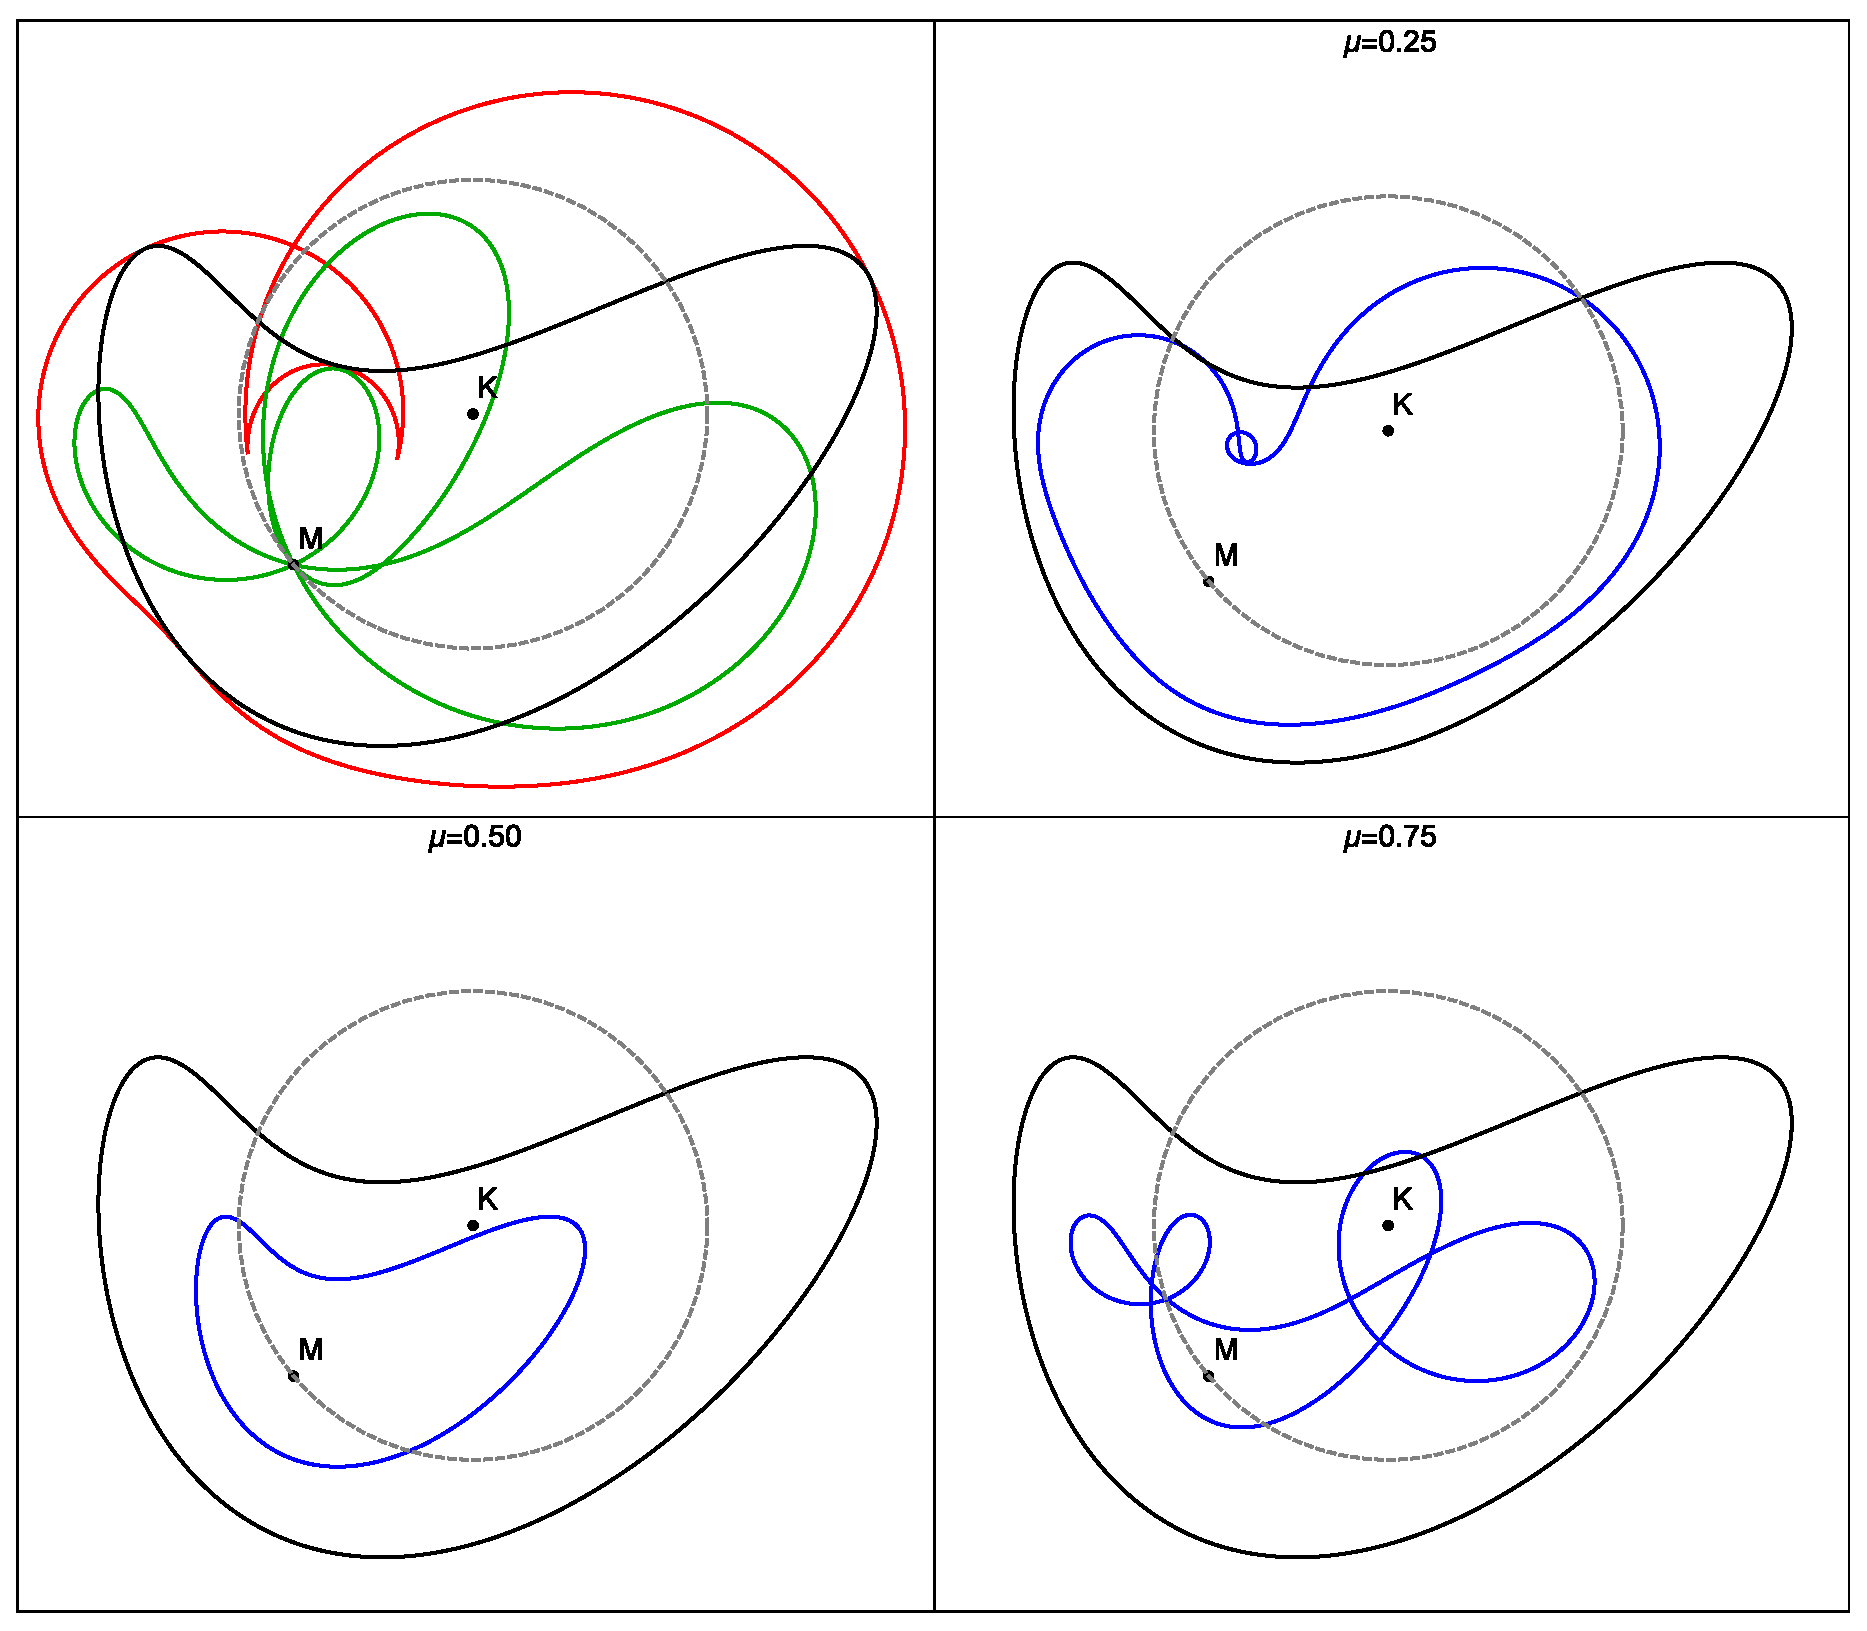
\includegraphics[width=\textwidth]{pics/0070_interpolated_concave.eps}
    \caption{\textbf{Top left}: a generic concave curve $\mathcal{C}$ (black) is shown as well as its curvature centroid $K$ and a circle about it where $M$ lies. Also shown are the pedal (red) and contrapedal (green) curves with respect to $M$. Note their areas are invariant for $M$ anywhere on a circle centered on $K$. \textbf{Top right, bottom left, bottom right}: the interpolated pedal curve (blue) for $\mu=0.25$, $0.5$, and $0.75$, respectively. Its area is also invariant for $M$ on a circle centered on $K$. Notice that at $\mu=0.5$ (bottom left) the interpolated pedal is homothetic (scale of 1/2) to $\mathcal{C}$ and its shape (and area) is independent of the location of $M$. Video of interpolated curve vs $\mu$: \href{
    https://youtu.be/0SW\_tBUeNKg}{\texttt{https://youtu.be/0SW\_tBUeNKg}}. Video of area invariance over circle for various $\mu$: \href{https://youtu.be/gR8Axe823\_M}{\texttt{https://youtu.be/gR8Axe823\_M}}}
    \label{fig:interp-concave}
\end{figure}
\label{sec:epilogue}

\section{Further Questions}
%\label{sec:conclusion}
One open question is whether a common thread exists which links the Steiner Hat \cite{garcia2020-deltoid}, the Hybrid, and Pseudo-Talbot curves, since all of them are area-invariant over $M$ on the ellipse. Furthermore, if a continuous family of curves exists with this area-invariance property. 
%Table~\ref{tab:videos} contains links to videos which illustrate some of the above phenomena. Column ``PL\#'' provides an index within a Youtube playlist.

\begin{table}[H]
\scriptsize
\begin{tabular}{|c|l|l|l|}
\hline
\href{youtu.be}{PL\#} & Title & Narrated \\
\hline
\href{youtu.be}{01} & 
\makecell[lt]{xxx} & no \\
\hline
\end{tabular}
\caption{Playlist of videos. Column ``PL\#'' indicates the entry within the playlist.}
\label{tab:videos}
\end{table}

%\section{Rotated pedal curve}
%\label{sec:rotated pedal}
%
The rotated pedal curve $\mathcal{E}_{\theta}$ is given by
$[X_\theta/\Delta,Y_\theta/\Delta]$ where:
\begin{align*}
 X_\theta &=  - 
  \left(     {a}^{2}  \sin^2  t   
\cos^2\theta +\frac{1}{2} a b\sin \left( 2\,\theta
 \right)  \sin \left( 2\,t \right) +  b^2  \cos^2 t 
  \sin^2\theta  
 \right) {x_0} \\
&+ \frac{1}{2} \left(  (b^2
  \cos^2 t   - {a}^{2} \sin^2t)\sin \left( 2\,\theta \right)
  +ab\sin
 \left( 2\,t \right) \cos \left( 2\,\theta \right)   \right)  y_0
 \\
 &+ \frac{b}{4}(c^2 \cos t \sin(2t) + 2 a^2 \sin{ t} )\sin(2\theta) - a \cos t (b^2\cos^2\theta + c^2\, \sin^2 t\sin^2\theta) 
 \\
 Y_\theta&= \frac{1}{2} \left( (  b^2  \cos^2t -   a^2\sin ^2{t} )  \sin(2\theta)+ a b  \sin (2t)  \cos(2  \theta)       \right)  x_0\\
 &+ \left(  (    a^2 \sin ^2{t}-b^2\cos^2t) \cos^2\theta   +\frac{1}{2} a b  \sin(2\theta)     \sin(2 t)  - a^2  \sin ^2{t}\right)  y_0\\
 &+  \frac{c^2}{4}  \left(2b \cos t\sin^2\theta+ a  \sin {t}   \sin(2\theta)    \right)  \sin(2 t) 
  -\frac{ab}{2}(2a \cos^2\theta  \sin {t}   +b \cos{t}  \sin(2\theta)  
   \\
 \Delta&={b}^{2}   \cos^2 t +{a}^{2}\sin^2t
\end{align*}

\begin{proposition}
The signed are of $\mathcal{E}_\theta$
is given by
\[\frac{\pi}{2}(2ab\cos^2\theta + (a - b)^2 + x_0^2 + y_0^2) \]
\end{proposition}

\section*{Acknowledgments}
We would like to thank Robert Ferréol and Mark Helman for their help during this work. We are also grateful to the referee's corrections and invaluable suggestions for improvement.

The second author is fellow of CNPq and coordinator of Project PRONEX/ CNPq/ FAPEG 2017 10 26 7000 508.

\appendix

\section{Evolutoids}
Some of the results in this section appear in \cite{jesus2015,jesus2014}. Consider a plane  curve $\mathcal{C}(t)=[x(t),y(t)]$ defined by a support function $h$, see Equation \eqref{eqn:support}.
 
The family of lines passing through $P(t)=[x(t),y(t)]$ making a constant angle $\theta$ with $(x^\prime(t),y^\prime(t)) $ is given by:

% simplificacao stachel (
\begin{align*}
 \mathcal{L}_{\theta}(t):&  \cos(\theta-t) \,x -  \sin(\theta-t)\, y - h(t) \cos\theta + h'(t)  \sin\theta = 0
\end{align*}

%\begin{align} 
%\mathcal{L}_{\theta}(t):& \left( \sin \left( 2\,\theta \right) +\sin \left( 2\,t \right) 
%\right) x+ \left( \cos \left( 2\,\theta \right) -\cos \left( %2\,t \right)  \right) y\\-&h(t)  (  \sin t + 
 %\sin \left( 2\,\theta+t \right) )+  h '(t)   (  \cos t %-\cos\left( 2\,\theta+t \right) )=0 \nonumber
%\end{align}

Let $\mathcal{C}_\theta(t)=(x_\theta,y_\theta)$ denote the envelope of $\mathcal{L}_\theta(t)$. This will be given by:

\begin{align*} x_{\theta}(t)=&\frac{1}{2}  \left( \cos \left( t-2\,\theta \right) + 
  \,\cos t  \right) h \left( t \right) -h'(t)\sin t    +\frac{1}{2} \left(\cos \left( t-2\,\theta 
  \right) - \,\cos t  \right)  h'' \left( t \right) \\
  %
  y_{\theta}(t)=&\frac{1}{2} \left(\sin \left( t-2\,\theta \right)  +
  \,\sin t \right) h(t)   +h'(t)\cos t    +\frac{1}{2} \left(\sin \left( t-2\,\theta 
  \right) - \,\sin t  \right)  h'' (t)
 \end{align*}

\noindent Note that $\mathcal{C}_{\pi/2}$ is the {\em evolute} of $\mathcal{C}$. Let $h_{\theta}(t)=h(t-\theta)\cos\theta +h'(t-\theta)\sin\theta$. Changing variables $t=t-\theta$ it follows that the envelope is  given by
  
\begin{align*}
  x_{\theta}(t-\theta)=&h_{\theta}(t)\cos t-h_{\theta}'(t)\sin t\\
  y_{\theta}(t-\theta)=&h_{\theta}(t)\sin t+h_{\theta}'(t)\cos t
\end{align*}
  
Let $S(.)$ denote the signed area of a curve. Then
  
  \begin{align*}
  S(\mathcal{C})=&\frac{1}{2} \int_0^{2\pi}( h(t)^2-h'(t)^2) dt\\
  S(\mathcal{C}_{\pi/2})=&\frac{1}{2} \int_0^{2\pi}( h'(t)^2-h''(t)^2) dt
  \end{align*}
  
 \begin{proposition}
 $S(\mathcal{C}_\theta)$ is given by
  	
  	\[ S(\mathcal{C}_\theta)= S(\mathcal{C})\cos^2\theta+S(\mathcal{C}_{\pi/2})\sin^2\theta\]
%\label{prop:area}
\end{proposition}

\begin{proof}
The signed area of the evolute $\mathcal{C}_{\pi/2}$ is negative in general, and zero if $\mathcal{C}$ is a circle. Integrating Equation~\ref{eqn:area} by parts and simplifying it yields the claim.
\end{proof}

%\begin{remark}
%From \cite{reventos_2007} we have that:
%	\[\int_{\mathcal{C}} \frac{ds}{k(s)}=2(A-A_e).\]
%\end{remark}

Let $L(.)$ denote the perimeter of a curve.

\begin{proposition}
For small $\theta$, $L(\mathcal{C}_{\theta}$) is given by:
	
	\[L(\mathcal{C}_{\theta} )=L(\mathcal{C})\cos{  \theta} \]
\end{proposition}

\begin{proof} Let $T,N$ define the tangent and normal axis of the Frenet frame. From \cite{giblin_2014} we have that
	\[  \mathcal{C}_{\theta}(s)=\mathcal{C}(s)+\frac{\cos\theta\sin\theta}{k(s)}T(s)+\frac{ \sin^2\theta}{k(s)}N(s).\]
	
Differentiating the above and using Frenet equations $T'={k}N$ and $N'=-{k}T$, it follows that
	
\[ \mathcal{C}_{\theta}'(s)=\frac{ k(s)  ^{2}\cos{\theta} -  k'(s)\sin{\theta}}{ k(s) ^{2}}  \left( N(s) \sin{\theta}+T(s) \cos{\theta} \right) 
	\]
	Therefore,
	\[ |\mathcal{C}_{\theta}'(s)|= |\cos\theta -\frac{k'(s)}{k(s)^2}\sin\theta| .\]
	
	For small $\theta$ it follows that
		\[ |\mathcal{C}_{\theta}'(s)|= \cos\theta -\frac{k'(s)}{k(s)^2}\sin\theta.\]
	Integration leads to the result stated.  
\end{proof}


\label{app:general-evolutoids}

%\clearpage

\section{Table of Symbols}
\begin{table}[!htbp]
\small
\begin{tabular}{|c|l|l|}
\hline
symbol & meaning & note \\
\hline
$\mathcal{E}$ & ellipse & semi-axes $a,b$\\
$\mathcal{K}_r$ & circle of radius $r$ concentric with $\mathcal{E}$ & \\
$M$ & a point in the plane & \\
$P(t)$ & a point on $\mathcal{E}$ & $[a\cos{t},b\sin{t}]$ \\
$\mathcal{L}(t)$ & line through $P(t)$ along $[P(t)-M]^\perp$ & \\
$Q_p,Q_{c},Q_{\theta}$ & pedal, contrapedal, rotated pedal feet & \\
$Q_{\mu}$ & linear interpolation of $Q_p,Q_{cp}$ & \\
$Q^*$ & intersection of pedal line with $\mathcal{L}(t)$ & \\
\hline
$\mathcal{E}_p$ & pedal curve of $\mathcal{E}$ wrt $M$ & locus of $Q_p$\\
$\mathcal{E}_{n}$ & negative pedal curve of $\mathcal{E}$ wrt $M$ & envelope of $\mathcal{L}(t)$ \\
$\mathcal{E}_{c}$ & contrapedal curve of $\mathcal{E}$ wrt $M$ & locus of $Q_{c}$  \\
$\mathcal{E}_{\theta}$ & rotated pedal curve of $\mathcal{E}$ wrt $M$ & locus of $Q_{\theta}$  \\
$\mathcal{E}_{\mu}$ & interpolated pedal curve of $\mathcal{E}$ wrt $M$ &  locus of $Q_{\mu}$ \\
$\mathcal{E}^*$ & hybrid pedal curve of $\mathcal{E}$ wrt $M$ & locus of $Q^*$ \\
$\mathcal{E}^\dagger$ & pseudo Talbot's curve of $\mathcal{E}$ wrt $M$ & locus of $Q^\dagger$ \\
\hline
$A$ & area of $\mathcal{E}$ & $\pi{a}{b}$ \\
$A_p,A_c,A_{\theta},A_\mu$ & areas of $\mathcal{E}_p,\mathcal{E}_c,\mathcal{E}_{\theta},\mathcal{E}_{\mu}$ & invariant for $M$ on a $\mathcal{K}_r$ \\
$A_n,A^*$ & areas of $\mathcal{E}_n,\mathcal{E}^*$ & invariant for $M$ on $\mathcal{E}$ \\
\hline
\end{tabular}
\caption{Symbols used.}
%\label{tab:symbols}
\end{table}

\label{app:symbols}
\newpage
\bibliographystyle{maa}
\bibliography{references,authors_rgk}

%\clearpage
%\section*{Response to Referee regarding BZAG-D-20-00147}
%\subsection{Structural modifications}

We added a sentence to the end of the abstract and introduction about the generalization of the result to smooth curves. Appendix B, following the referee's suggestion, was promoted to Section 5.

\subsection{Singularity (Remark 1)}
The concept of singularity we are using is that of parametric curves, i.e., a point $t_0$ of a smooth curve $\alpha(t)$ is called singular when $\alpha'(t_0)=0$. This definition, in general, differs from that of implicit curves $f(x,y)=0$. For example, self-intersections in parametric curves are always singularities of the implicit curve. We derived the implicit equation (as suggested by the referee) of a $\theta$-evolutoid; in general the curve is of degree 12. In several examples  it is of degree 6.
\subsection{$\theta$-evolutoid}

New redaction to Remark 1.

\textcolor{blue}{ 
\begin{remark*}
 The parametrization $[x_\theta(t), y_\theta(t)]$ of the $\theta$-evolutoid will   have 4, 2, or 0 singularities if
$\theta\in(\theta_0,\pi-\theta_0)$, $\theta\in\{\theta_0,\pi-\theta_0\}$, or $\theta\notin[\theta_0,\pi-\theta_0]$, respectively. Moreover, the ${\theta_0}$-evolutoid is singular at $t_1=\frac{3\pi}{4}$ and
	$t_2=  \frac{7\pi}{4}$.
	Here, a  point $t=t_0$ is called singular when $x'_\theta(t_0)=y'_\theta(t_0)=0$.
	These points correspond to real cusps of the curve.  
	In the implicit form,   a  $\theta$-evolutoid is given by $f^{-1}(0)$, and $f$ being a polynomial   function of degree 12.
\end{remark*}
}
\subsection{Note on page 5} We removed the note below, note it is never used in the article: (note we will use red to denote excerpts removed from the text)

\textcolor{red}{  
Note: when expressed in line coordinates, the cusps of the evolute are regular. Specifically, cusps of the evolute are inflection points of its dual % \cite{fischer2001,akopyan2007-conics}. 
}

\subsection{The equation of $\mathcal{E}_\theta$ is not given}

Inserted parametrization of $\mathcal{E}_{\theta}$ as asked. (blue means inserted)

\textcolor{blue} { 
The rotated pedal curve $\mathcal{E}_{\theta}$ is given by
$[X_\theta/\Delta,Y_\theta/\Delta]$ where:
{\small 
\begin{align*}
 X_\theta &=  - 
  \left(     {a}^{2}  \sin^2  t   
\cos^2\theta +\frac{1}{2} a b\sin \left( 2\,\theta
 \right)  \sin \left( 2\,t \right) +  b^2  \cos^2 t 
  \sin^2\theta  
 \right) {x_0} \\
&+ \frac{1}{2} \left(  (b^2
  \cos^2 t   - {a}^{2} \sin^2t)\sin \left( 2\,\theta \right)
  +ab\sin
 \left( 2\,t \right) \cos \left( 2\,\theta \right)   \right)  y_0
 \\
 &+ \frac{b}{4}(c^2 \cos t \sin(2t) + 2 a^2 \sin{ t} )\sin(2\theta) - a \cos t (b^2\cos^2\theta + c^2\, \sin^2 t\sin^2\theta) 
 \\
 Y_\theta&= \frac{1}{2} \left( (  b^2  \cos^2t -   a^2\sin ^2{t} )  \sin(2\theta)+ a b  \sin (2t)  \cos(2  \theta)       \right)  x_0\\
 &+ \left(  (    a^2 \sin ^2{t}-b^2\cos^2t) \cos^2\theta   +\frac{1}{2} a b  \sin(2\theta)     \sin(2 t)  - a^2  \sin ^2{t}\right)  y_0\\
 &+  \frac{c^2}{4}  \left(2b \cos t\sin^2\theta+ a  \sin {t}   \sin(2\theta)    \right)  \sin(2 t) 
  -\frac{ab}{2}\left(2a \cos^2\theta  \sin {t}   +b \cos{t}  \sin(2\theta)  \right)
   \\
 \Delta&={b}^{2}   \cos^2 t +{a}^{2}\sin^2t
\end{align*}
}
}

\subsection{Typo in Proposition 1}

Removed 
 \textcolor{red} {
 \[ S_{\theta}=\pi\,ab   \cos^2   \theta  -  \,{\frac {3
		    c^{2} }{8ab}}\sin^2  \theta   
\]
}
 
Inserted, changing $c^2 \rightarrow c^4$.

\textcolor{blue}{ 
\[S_{\theta}=\pi a b \cos^2\theta -\frac{  3 c^4\pi}{8 ab} \sin^2\theta\]
}

\subsection{Proposition 4: mistake in formula}

The source of the error was that calculations were done with $ \mu$ instead of $(1-\mu)$. Remove:
\textcolor{red}{\begin{align*} A_{\mu}=& \left(2\,{a}^{2}-3\,ab+2\,b^{2}+2\,x_0^{2}+2\,y_0^{2} \right) \pi\,{\mu}^2 -2\,\left( (a-b)^2  +x_0^{2}
+y_0^{2} \right) \pi\,\mu \\
+&\frac{1}{2}\left( (a-b)^2 +x_0^{2}+y_0^{2} \right) \pi\\
  =&(2\mu-1)[(1-\mu) A_p-\mu A_c]+\mu(1-\mu)A. 
\end{align*}
}

Inserted the following corrected expression:

\textcolor{blue}{ 
\begin{align*}
A_{\mu}=& \left(2\,{a}^{2}-3\,ab+2\,b^{2}+2\,x_0^{2}+2\,y_0^{2} \right) \pi\,{\mu}^2 -2\,\left( (a-b)^2  +x_0^{2}
+y_0^{2} \right) \pi\,\mu \\
+&\frac{1}{2}\left( a^2+b^2 +x_0^{2}+y_0^{2} \right) \pi\\
  =&(1-2\mu)[(1-\mu) A_p-\mu A_c]+\mu(1-\mu)A. 
\end{align*}
}

\subsection{Theorem 3: corrected the sign}
  
 \textcolor{blue}{
 	\[ A^\dagger=  -  \frac {\pi\, \left( 3\,{a}^{4}+2\,{a}^{2}{b}^{2}+3\,{b}^{4}
 \right)  \left( {a}^{2}-2\,ab-{b}^{2} \right)  \left( {a}^{2}+2\,ab-{
b}^{2} \right) }{8 a^{3} b^{3}}
	\]
 }
 \subsection{Evolutoids}
 Referee says: ``An additional mistake must have happened in the equations for the evolutoids''. Solution: there is a typo in the equation of the family $\mathcal{L}_{\theta}(t)$ (below, removed)

\textcolor{red}{ 
\begin{align*} 
\mathcal{L}_{\theta}(t):& \left( \sin \left( 2\,\theta \right) +\sin \left( 2\,t \right) 
\right) x+ \left( \cos \left( 2\,\theta \right) -\cos \left( 2\,t
\right)  \right) y\\
-&h(t)  (  \sin t - 
 \sin \left( 2\,\theta+t \right) )+  h '(t)   (  \cos t -\cos
\left( 2\,\theta+t \right) )=0
\end{align*}
}

Inserted the following correction (blue below):   

In the report, we think that the referee computed with angle $-\theta$. This is a choice of orientation.  See Fig. below.

 The equation \eqref{eq:line-theta} can be simplified as:
\textcolor{blue}{
\[ 
 \mathcal{L}_{\theta}(t):   \cos(\theta-t) \,x -  \sin(\theta-t)\, y - h(t) \cos\theta + h'(t)  \sin\theta = 0 \]
 }

Therefore we think we should maintain the two expressions below as in the original (see Figure~\ref{fig:referee}. Let $\mathcal{C}_\theta(t)=(x_\theta,y_\theta)$ denote the envelope of $\mathcal{L}_\theta(t)$. This will be given by:
 
\begin{align*} x_{\theta}(t)=&\frac{1}{2}  \left( \cos \left( t-2\,\theta \right) + 
  \,\cos t  \right) h \left( t \right) -h'(t)\sin t    +\frac{1}{2} \left(\cos \left( t-2\,\theta 
  \right) - \,\cos t  \right)  h'' \left( t \right) \\
  %
  y_{\theta}(t)=&\frac{1}{2} \left(\sin \left( t-2\,\theta \right)  +
  \,\sin t \right) h(t)   +h'(t)\cos t    +\frac{1}{2} \left(\sin \left( t-2\,\theta 
  \right) - \,\sin t  \right)  h'' (t)
 \end{align*}
 
  

 \begin{figure}[H]
     \centering
     \includegraphics[scale=0.5]{pics/figura_gerada_curva_referee.png}
     \caption{Curve produced with  $\theta=-\pi/3$ and lines with $t=\pi/4$ (red) and $t=-\pi/4$ (blue). Support function $h(t)=2\cos^2(t) + 3\sin^2(t)$ as in the report. The curve was drawn taking into account  the correction of a typo in equation of $\mathcal{L}_{\theta}$. Note our $\theta$ is equal to $-\theta$ of referee's equations obtained in the report.}
     \label{fig:referee}
 \end{figure}
 
 %\textcolor{blue}{ reconferi calculos e esta ok essa equacao acima.
 %
 %}
 

 \subsection{ Negative pedal curve}
 
 %$\bullet $  {\bf Negative pedal curve}
 
Recall $\mathcal{E}^\dagger$ is the negative pedal curve of $\mathcal{E}^*$ (Section~\ref{sec:intro} and Figure~\ref{fig:hybrid-npc}). For $M=[a\cos u,b\sin u]$ on the ellipse, the coordinates $[x^\dagger,y^\dagger]$ of $\mathcal{E}^\dagger$ can be derived explicitly. Recall the original equation (below):
\textcolor{red}{{\small
\begin{align*}
x^{\dagger}(u)=&-{\frac { \left( \left(  k_x+1 \right) {a}^{4}-2
 \left(k_x+1\right) {b}^{2}{a}^{2}+ k_x b^4  \right)\cos u
}{{b}^{2}a}}\\
-&2\,{\frac { \left( {a}^{2}-{b}^{2} \right) ^{2}   
\sin^{3}t \cos{t}\sin{u}}{{b}^{2}a}} 
 + \frac {\cos t \left( {a}^{2}+{b
}^{2} \right)  \left( -{a}^{2} \sin^2t-{b}^{2} \cos^2t+2\,{b}^{2}
 \right) }{{b}^{2}a}\\
 y^{\dagger}(u)=&-2\,{\frac { \left( {a}^{2}-{b}^{2} \right) ^{2}\sin t
 \cos^3{t}  \cos u}{{a}
^{2}b}}-{\frac { \left(  \left(k_y-1 \right) {a
}^{4}-2 k_y {b}^{2}{a}^{2}+
 k_y {b}^{4} \right) \sin u}{{a}^{2}b}}\\
 +&{\frac {\sin t \left( {a}^{2}+{b
}^{2} \right)  \left( ({a}^{2}-b^2) \cos^2t+{a}^{2} \right) 
}{{a}^{2}b}}\\
k_x=&2\cos^4t-3\, \cos^2t\\
k_y=&2\cos^{4}t- \cos^2t
\end{align*}
}
}

We have replaced the above by the following simplified expression

\textcolor{blue}
{\small  
\begin{align*}
x^{\dagger}(u)=&\frac{\left(c^4(2\cos(2t) - \cos(4t)) - (a^2 - 3b^2)(a^2 + b^2)\right)\cos{u} }{4 a b^2} - \frac{2c^4 \sin^3t \cos{t} \sin{u}}{a b^2}\\
&+ \frac{(a^2 + b^2)(b^2-c^2\sin^2{t}  )\cos{t}}{a b^2}\\
y^{\dagger}(u)=&-\frac{2c^4 \sin{t} \cos^3{t}\cos{u}}{a^2b} - \frac{(c^4(2\cos(2t) + \cos(4t)) - (3a^2 - b^2)(a^2 + b^2))\sin{u}}{ 4a^2b}\\
&+\frac{  (a^2 + b^2)(c^2 \cos^2{t}    + a^2)\sin{t}}{a^2 b}
\end{align*}
}
\subsection{Comments about Proposition 9 (originally in App B)}
  
First of all it was moved with the appendix to section 5. It is now Proposition 7. It is derived using the parametrization by the support function. Note the change of $2 \mu-1 \rightarrow  1-2\mu$. Now it reads>
 
 \textcolor{blue}{\textbf{Proposition 7}: For any smooth regular closed curve $\mathcal{C}$ with non-zero rotating index, the isocurves of $A(\mathcal{C}_\mu)$ are circles centered on $K$.
In fact, \[A(\mathcal{C}_\mu) =(1-2\mu)[(1-\mu) A(P_M)-\mu A(C_M)]+\mu(1-\mu)A(\mathcal{C}).\] 
 }

\subsection{Example 1 }
An example was introduced to better explain Fig. 11. An update of the   Figure  and a video were produced. Also added two video links at the end of the figure's caption which illustrate continuous interpolation and area invariance over a circle centered on K. The curve used in the example is shown here for reference in Figure~\ref{fig:convex-curve}, here is a copuy of the example already in the text:

\textcolor{blue}{
  Consider the non convex smooth curve 
\[ 
\mathcal{C}(t)= [  2 \cos t -\frac{1}{4}\sin( 2t) + \frac{3}{10}\cos(2t),
\sin{t} + \frac{3}{4}\cos(2t)] \] 
The curvature centroid of $\mathcal{C}$ is $K=[0.1823\ldots, 0.01943\ldots]$. The  centroid
$[\int xds/\int ds, \int yds/\int ds]$ is the point $[0.1387\ldots, -0.2504\ldots ] $ and the center of mass $[\int xdxdy/\int dxdy, \int ydxdy/\int dxdy]$ is $[12/95, 7/19]=[0.1263\ldots, -0.3684\ldots]$.
}

   \begin{figure}[H]
       \centering
   \includegraphics[scale=0.3]{pics/figura11.png}
       \caption{Non convex curve with curvature centroid  $K=[0.1823\ldots, 0.01943\ldots]$.}
       \label{fig:convex-curve}
   \end{figure}


\subsection{Corollary 6} The proof of Corollary 6 was reformulated and a remark for convex curves was added.


\textcolor{blue}{\textbf{Corollary 6} The family of isocurves of $A(P_M)$ and $A(C_M)$ are circles centered at
\begin{align*}
\label{eq:centroK}
K_0=\left[	\frac{1}{\pi} \int_0^{2\pi}\!\!\!\!\! h(t)\cos t \,dt,	\frac{1}{\pi} \int_0^{2\pi}\!\!\!\!\! h(t)\sin t \, dt\right]
\end{align*}
}

\textcolor{blue}{\begin{proof}  Consider the mean $K_0=\frac{1}{2\pi}\int_0^{2\pi}\mathcal{C}(t)dt$ of the curve $\mathcal{C}$ given by Equation \eqref{eqn:support}. Integration by parts leads to the result stated. Expressions of the areas $A(P_M)$ and $A(C_M)$ given in Equation \eqref{eqn:apm-acm} shows that the isocurves are cirles centered at $K_0$.
\end{proof}
}

We also added the following remark

\textcolor{blue}{\textbf{Remark: } For convex curves,  $K_0$ coincides with the   centroid of Steiner $K$ given by Equation \eqref{eqn:steiner-k}. In fact, using the parametrization  of the curve $\mathcal{C}$ given by Equation \eqref{eqn:support} it follows that $ds= |h(t)+h''(t)|dt$ and $k(t)=1/(h(t)+h''(t))$. Integration by parts leads to the result.}


\end{document}